\documentclass[a4paper, 12pt, article]{memoir}

\usepackage{fullpage}
\setlength{\footmarkwidth}{0em}
\setlength{\footmarksep}{0em}
\setlength{\thanksmarkwidth}{0em}
\setlength{\thanksmarksep}{0em}

\usepackage{fontspec}
\usepackage{amsmath}
\usepackage[tracking=true, nopatch=footnote]{microtype}
\usepackage{scalefnt}
\usepackage{csquotes}
\usepackage[main=brazil]{babel}

\usepackage{graphicx}
\usepackage{subcaption}
\usepackage{tikz} %for all basic options
\usepackage{tikz-qtree} %for simple tree syntax
\usepgflibrary{arrows} %for arrow endings
\usetikzlibrary{positioning,shapes.multipart} %for structured nodes
\usetikzlibrary{tikzmark}
\usepackage{tikz-qtree}
\usepackage{tree-dvips}
\usepackage{booktabs}
\usepackage{longtable}
\usepackage{array}
\usepackage{multirow}
\usepackage{wrapfig}
\usepackage{float}
\usepackage{colortbl}
\usepackage{pdflscape}
\usepackage{tabu}
\usepackage{threeparttable}
\usepackage{threeparttablex}
\usepackage[normalem]{ulem}
\usepackage{makecell}
\usepackage{xcolor}

\newcommand{\Bernoulli}{\text{Bernoulli}}
\newcommand{\LogNormal}{\text{LogNormal}}
\newcommand{\Normal}{\text{Normal}}
\newcommand{\Dirichlet}{\text{Dirichlet}}
\newcommand{\Exponencial}{\text{Exponencial}}
\newcommand{\logit}{\text{logit}}
\newcommand{\Dist}{\text{Dist}}
\newcommand{\Cop}{\text{Cop}}
\newcommand{\Sent}{\text{Sent}}
\newcommand{\Auth}{\text{Auth}}
\newcommand{\PoS}{\text{PoS}}
\newcommand{\Th}{\text{Th}}
\newcommand{\Dia}{\text{Dia}}
\newcommand{\abar}{\overline{\alpha}}
\newcommand{\bbar}{\overline{\beta}}
\newcommand{\bv}[1]{\beta_\text{#1}}
\newcommand{\bvi}[1]{\beta_{\text{#1}_i}}

\setmainfont{Gentium Plus}
\setmonofont[Scale=0.8]{Noto Sans}

\babelprovide[import, onchar=ids fonts letters]{ancientgreek}
% \babelfont[ancientgreek]{rm}{Brill}
\babeltags{grc = ancientgreek}

\usepackage{hyperref}
\usepackage{linguex}
\setlength{\Exlabelsep}{0.5em}
\setlength{\SubExleftmargin}{1.5em}
\usepackage{paralist}
\usepackage{hyphenat}
\hyphenation{
  Κυ-ρι-α-κί-δη
  Θεσ-σα-λο-νί-κη
}

\usepackage[normalem]{ulem}
\RequirePackage{xcolor}
\definecolor{green}{RGB}{16,87,87} % rgb(16,87,87)
\definecolor{red}{RGB}{193, 11, 105} % rgb(193, 11, 105)
\definecolor{yellow}{RGB}{218,222,104} % rgb(218,222,104)
\definecolor{pink}{RGB}{243,179,145} % rgb(243,179,145)
\definecolor{blue}{RGB}{161,184,206} % rgb(161,184,206)

\RequirePackage{hyperref}%
\hypersetup{%
	colorlinks=true, % false: boxed links; true: colored links
	linkcolor=green,  % color of internal links
	citecolor=green,  % color of links to bibliography
	filecolor=green,  % color of file links
	urlcolor=green,
}

\usepackage[
  backend=biber,
  uniquename=init,
  giveninits,
  dashed=true,
  style=authoryear-comp
  ]{biblatex}
\addbibresource{./biblio.bib}


\title{Rethinking case attraction on Ancient Greek infinitive clauses}
\author{
  Caio B. A. Geraldes\thanks{
		This research was funded by the 
	 The São Paulo Research Foundation (Fapesp), grant number 2021/06027-4.}
	\\\smallskip
	Universidade de São Paulo
	\\\smallskip
	<\href{mailto:caio.geraldes@usp.br}{\texttt{caio.geraldes@usp.br}}>
}
\date{June 25, 2025}

\begin{document}

\maketitle

\ex.
\a.συμβουλεύει \textbf{τῷ Ξενοφῶντι ἐλθόντα} {εἰς Δελφοὺς}
ἀνακοινῶσαι {τῷ θεῷ} {περὶ τῆς πορείας}.\\
Ele aconselha Xenofonte ir a Delfos e interrogar o deus sobre a viagem.
(Xen.\ \emph{Anab.} 3.1.5)
\b.ἀφῆκε \textbf{μοι ἐλθόντι} {πρὸς ὑμᾶς} λέγειν τἀληθῆ.\\
Ele me permitiu vir frente a vós dizer a verdade.
(Xen.\ \emph{Hell.} 6.1.13)


\noindent Trabalhos mencionados:
\textcite{Lancelot1658,Lancelot1709},
\textcite{Lakoff1970}, \textcite{Andrews1971}, \textcite{Quicoli1982},
\textcite{Spyropoulos2005}, \textcite{Tantalou2003},
\textcite{Sevdali2006,Sevdali2013}

\paragraph{Fonte dos dados:}  Diorisis Corpus
(\cite{TheDiorisisAncientGreekCorpus,diorisis2021}) with help of the project's
querying tool, Diorisis Search (\cite{DiorisisSearch}).

\paragraph{\emph{Corpus}:} Sentenças coletadas a partir das fontes literárias áticas e
Heródoto.

\paragraph{Ferramentas:} R (\cite{R}) com o os pacotes
\texttt{tidyverse} (\cite{tidyverse}), \texttt{dagitty} (\cite{dagitty}),
\texttt{ggdag} (\cite{ggdag}) e \texttt{rethinking} (\cite{McElreath2020}),
bem como o software Stan~(\cite{StanReferenceManual,StanUserGuide}).

\paragraph{Modelo tipológico:} \textcite{Corbett2006}

% \begin{compactitem}
% 	\item Case attraction as agreement
% 	\item Agreement defined as covariation of features in the pair of constituents
% 		containing a controller and a target in a given domain.
% 	\item Case attraction is the covariation of the feature $[Case]$ between the
% 		oblique object of a matrix clause and a predicate or attributive participle,
% 		adjetive or noun pertaining to an infinitive clause governed by the matrix'
% 		verb.
% 	\item The lack of case agreement (predicate in accusative) is the canonical
% 		agreement.
% 	\item Case attraction is a non\hyp{}canonical agreement resolution:
% 		\begin{compactitem}
% 		\item Its feature is non\hyp{}canonical.
% 		\item The agreement is optional (target is ``trigger happy'').
% 		\item Non-locality (interclausal).
% 		\end{compactitem}
% 	\item Typologically, when canonical and non\hyp{}canonical agreement
% 		resolutions, the later tends to be conditioned by features of the
% 		controller, domain, and target. Known conditions include:
% 		\begin{compactitem}
% 			\item class of predication (i.e.:\ class of the domain) via the Agreement
% 				Hierarchy (\cite{Corbett1979}).
% 			\item semantic features of the controller (thematic role).
% 			\item relative order of target and controller.
% 			\item Part of speech of target via the Predicate Hierarchy
% 				(\cite{Comrie1975}).
% 			\item Distance between controller and target (e.g.:~\cite{Levin2001}).
% 		\end{compactitem}
% \end{compactitem}
%
% \noindent Directed Acyclic Graph (\cite{Pearl2009}) for non\hyp{}canonical
% agreement according to~\textcite{Corbett2006}, with \textbf{A}greement,
% \textbf{C}ontroller, \textbf{D}omain, and \textbf{T}arget:
%
\begin{center}
  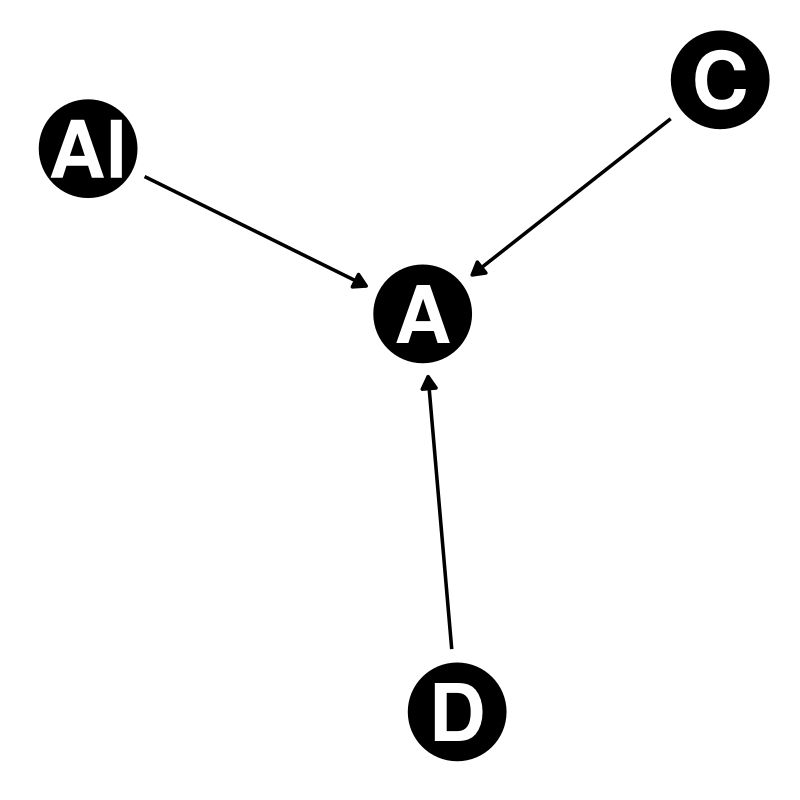
\includegraphics[width=0.40\textwidth]{../fala/plots/dag_non_canonical_agreement.png}
\end{center}

% \noindent The three main factors previously shown to correlate to case attraction:
% \begin{compactitem}
% 	\item Copular infinitives imply a different domain of agreement, as they
% 		select different predication classes;
% 	\item Main verbs with semantic modality imply a different type of controller,
% 		as they have higher subjecthood;
% 	\item Word order and distance imply different status for the target, as
% 		targets more to the left of the sentence are both structurally closer to the
% 		controller and have a higher communicative function.
% \end{compactitem}
%
\paragraph{Infinitivos copulares:} ver~\textcite{KG}

\ex. Agreement and Predicate Hierarchies~(\cite[233]{Corbett2006}):\\
\begin{tikzpicture}[baseline=0pt]
  \node (attr) at (0, 0) {Attributive};
  \node (pred) at (2.5, 0) {Predicative};
  \node (predv) at (2.9, -0.4) {Verb};
  \node (predp) at (3.5, 1) {Participle};
  \node (preda) at (5, 2) {Adjective};
  \node (predn) at (7, 2.5) {Noun};
  \node (relp) at (5.6, 0) {Relative Pronoun};
  \node (perp) at (9.1, 0) {Personal Pronoun};
  \node (less) at (0, -1) {-};
  \node (plus) at (9.1, -1) {+};
  \draw[->, thick] (attr) to (pred);
  \draw[->, thick] (pred) to (relp);
  \draw[->, thick] (relp) to (perp);
  \draw[->, thick] (pred) to (predp);
  \draw[->, thick] (predp) to (preda);
  \draw[->, thick] (preda) to (predn);
  \draw[->] (less) to (plus);
  \draw[->] (plus) to (less);
  \node at (4.5, -1.5) {Likelihood of agreement with semantic justification};
\end{tikzpicture}


\paragraph{Verbos impessoais:} ver~\textcite{Humbert1945}

% \textbf{Issue:} δοκέω has a rather low number of examples attesting
% attraction.

\paragraph{Verbos com semântica modal:} verbos como ἐξαρκεῖ e ἔξεστί tem maior
probabilidade de apresentar atração de caso
(\cite{Geraldes2020,Geraldes2025}).

% \noindent They do not assign thematic role to the controller, as
% in~\ref{gloss:mod}

\ex.\label{gloss:mod} ἀλλ᾽ ἐξαρκῇ σοι τὰ ἔργα αὐτῶν ὁρῶντι σέβεσθαι καὶ τιμᾶν τοὺς θεούς.\\
Mas é suficiente a ti observar as ações e respeitar e honrar os deuses.
(Xen.\ \emph{Mem.} 4.3.13)




\paragraph{Autoria e dialeto:} \textcite{Geraldes2020,Geraldes2025} mostra que o
uso de verbos com semântica modal são mais frequentes em diálogos filosóficos
que textos historiográficos.

\paragraph{Ordem de palavra e distância:} maiores distâncias diminuem a
probabilidade de atração de caso. Alvos que antecedem o controlador parecem
exigir atração de caso como no exemplo~\ref{gloss:prec}.

\ex.\label{gloss:prec}ὡς \textbf{ἀγαθοῖς} τε \textbf{ὑμῖν} προσήκει εἶναι.\\
Que vos seja dado ser boa gente. (Xen.\ \emph{Anab.} 3.2.11)




\begin{figure}[hbt]
  \centering
  \begin{minipage}{.45\textwidth}
    \begin{center}
      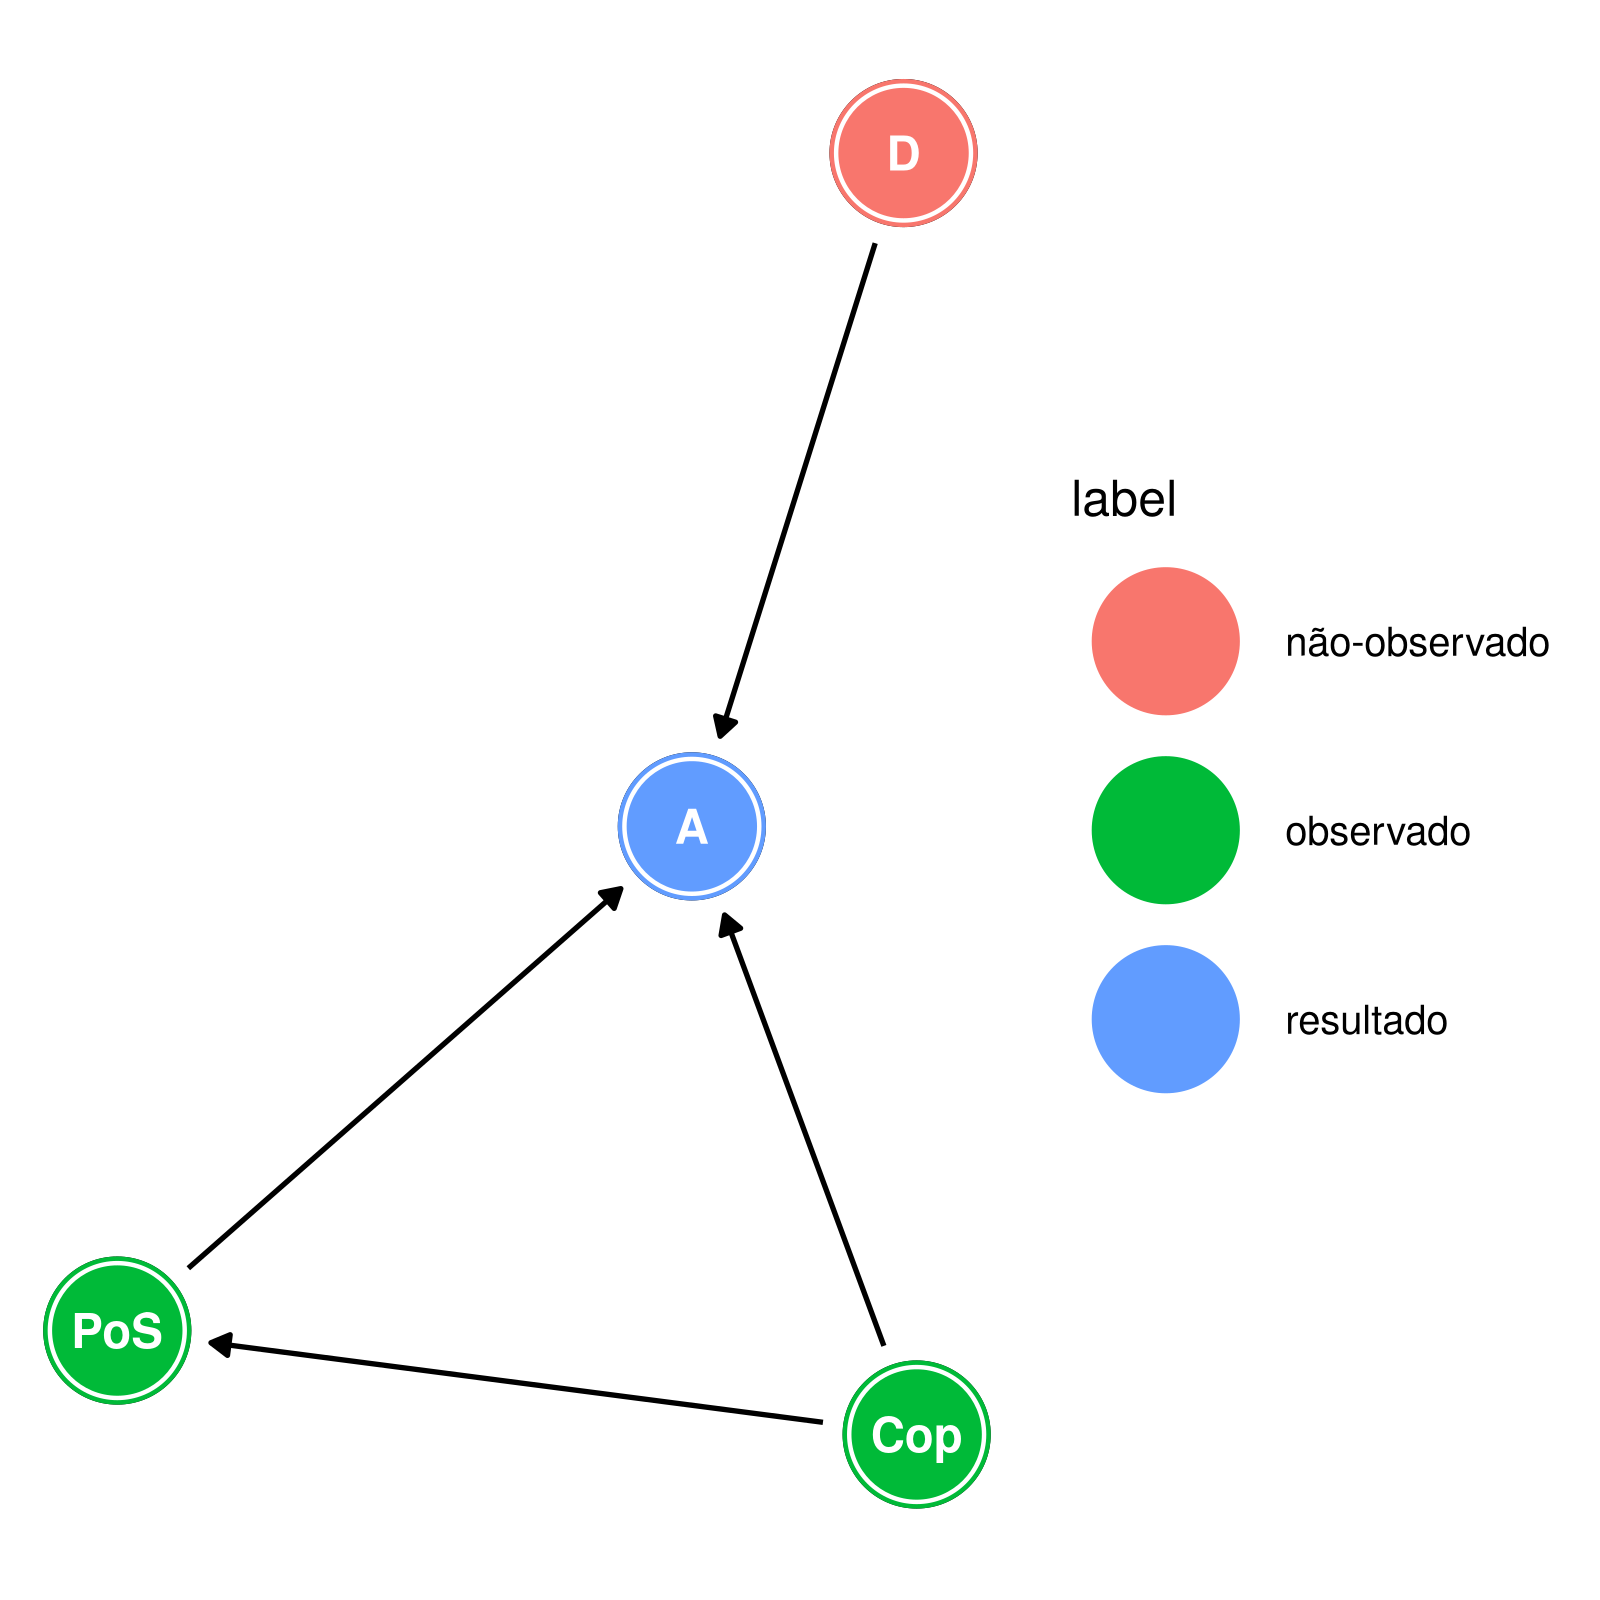
\includegraphics[width=\linewidth]{../fala/plots/dag_a.png}
    \end{center}
    \caption{DAG with \textbf{A}ttraction, \textbf{D}omain,
      \textbf{P}art \textbf{o}f \textbf{S}preech and \textbf{C}opula}\label{fig:dag_a}
  \end{minipage}
  \hfill
  \begin{minipage}{.45\textwidth}
    \begin{center}
      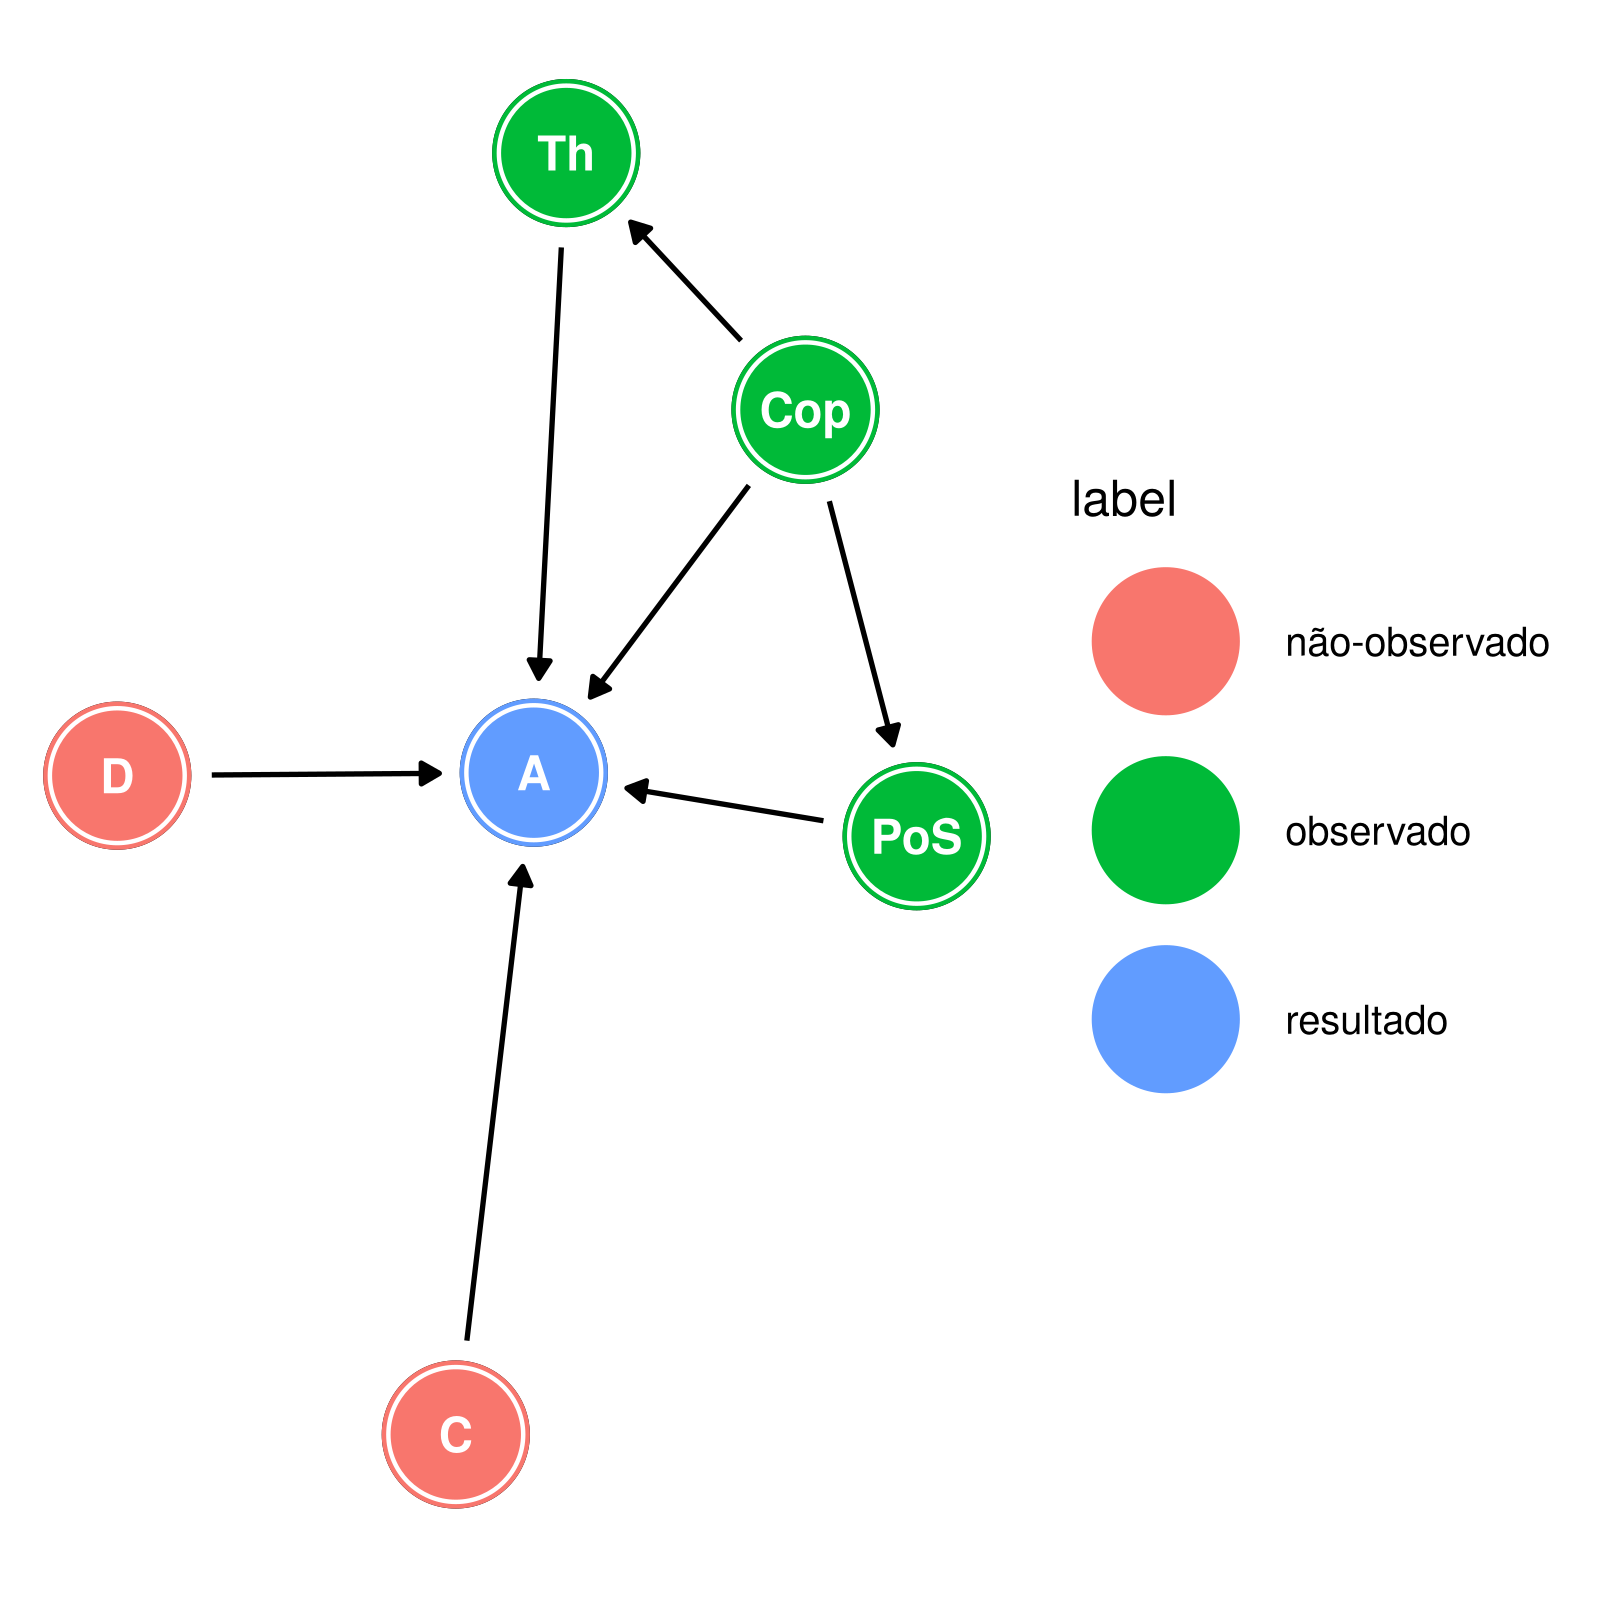
\includegraphics[width=\linewidth]{../fala/plots/dag_b.png}
    \end{center}
    \caption{DAG with \textbf{A}ttraction, \textbf{D}omain, \textbf{C}ontroller
      \textbf{P}art \textbf{o}f \textbf{S}preech, \textbf{C}opula and
      \textbf{Th}ematic role.}\label{fig:dag_b}
  \end{minipage}
\end{figure}

\begin{figure}[hbt]
  \centering
  \begin{minipage}{.45\textwidth}
    \begin{center}
      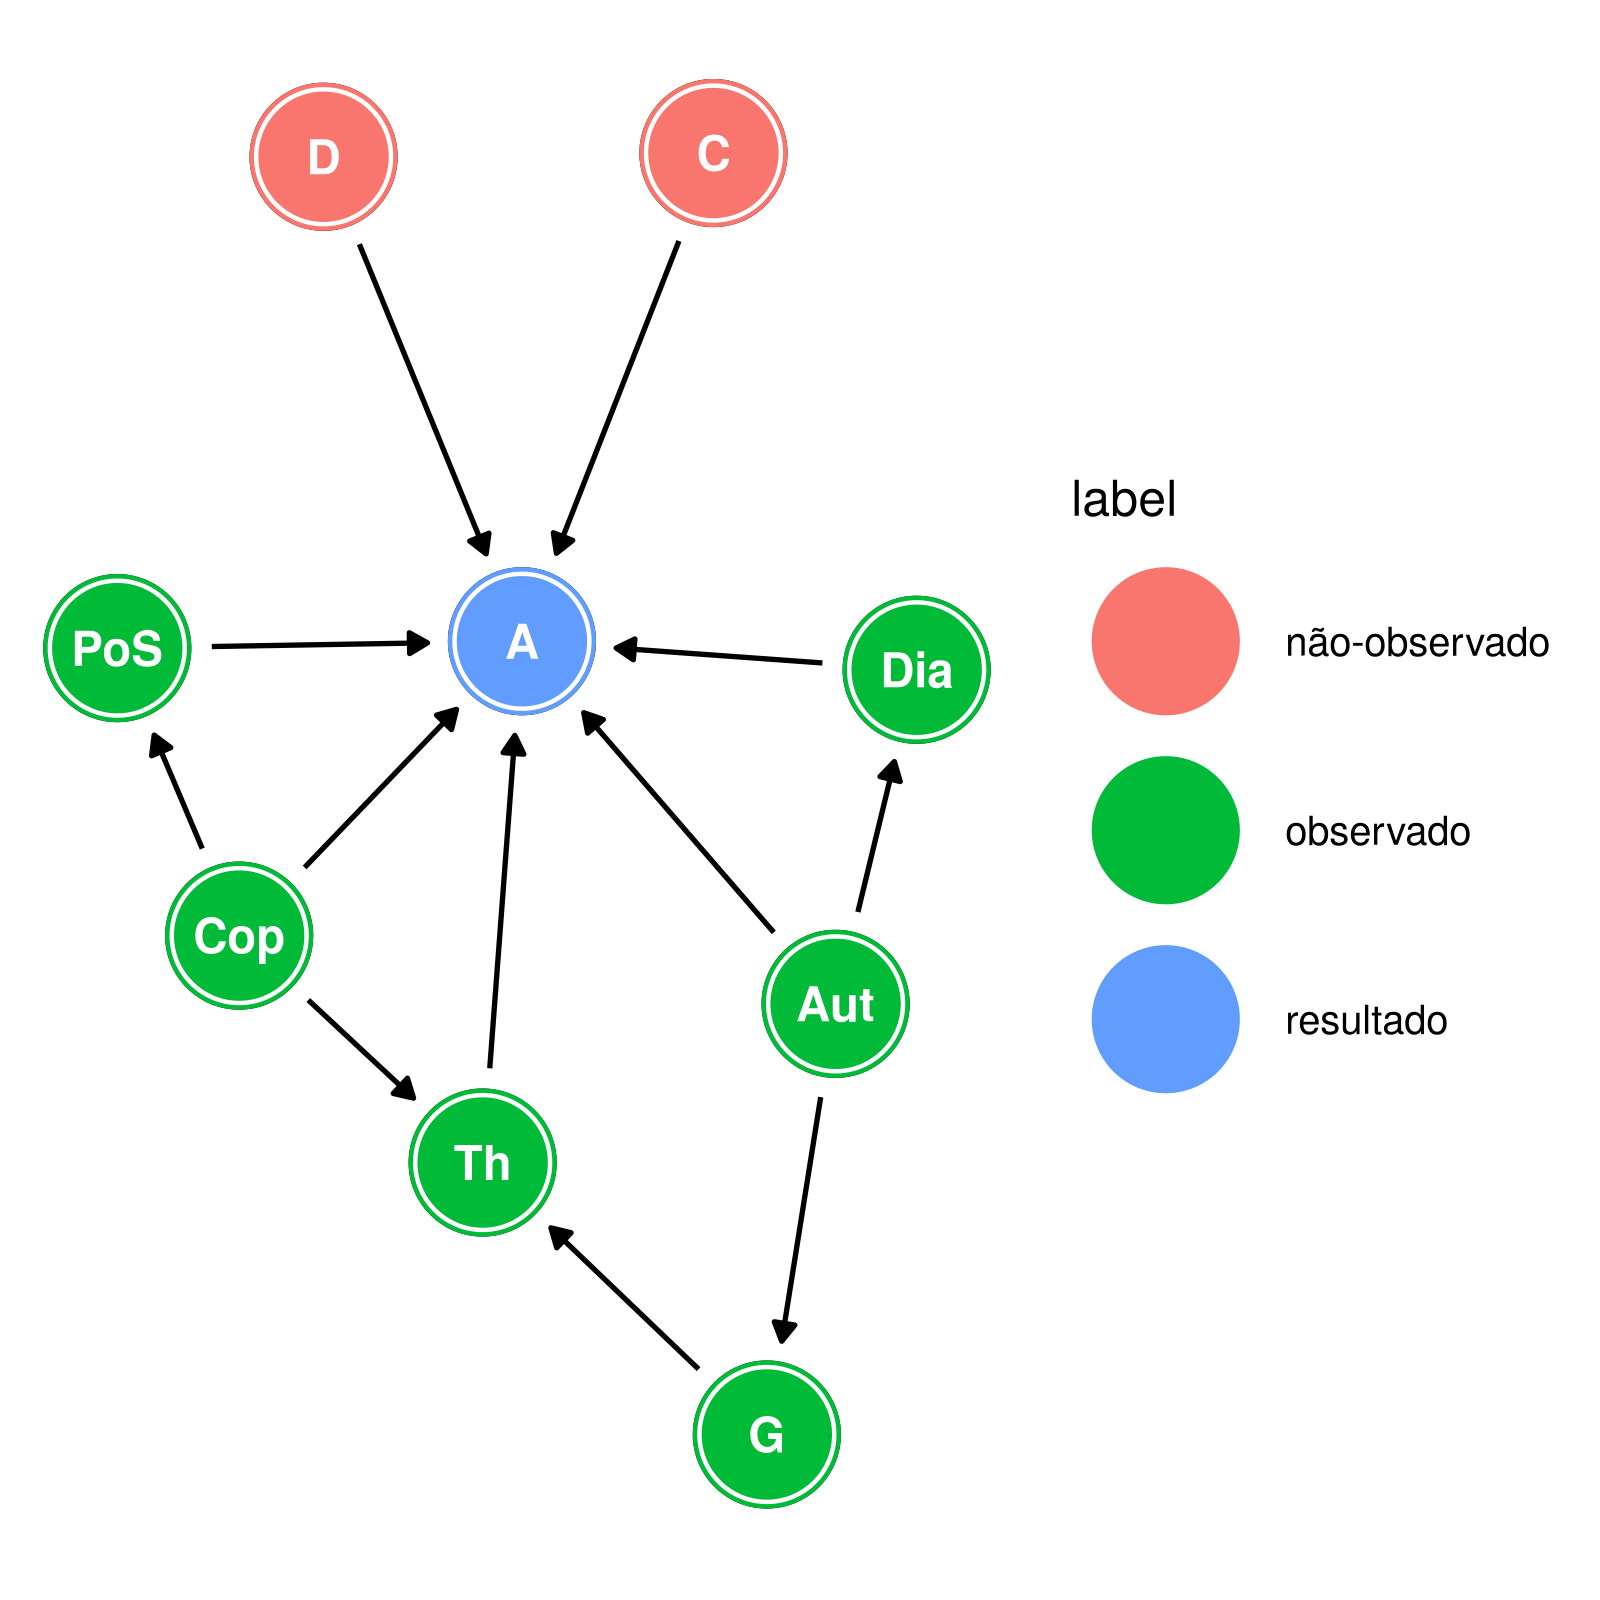
\includegraphics[width=\linewidth]{../fala/plots/dag_c.png}
    \end{center}
    \caption{DAG with \textbf{A}ttraction, \textbf{D}omain, \textbf{C}ontroller
      \textbf{P}art \textbf{o}f \textbf{S}preech, \textbf{C}opula,
      \textbf{Th}ematic role, \textbf{Auth}orship, \textbf{Genre}, and
      \textbf{Dia}lect.
    }\label{fig:dag_c}
  \end{minipage}
  \hfill
  \begin{minipage}{.45\textwidth}
    \begin{center}
      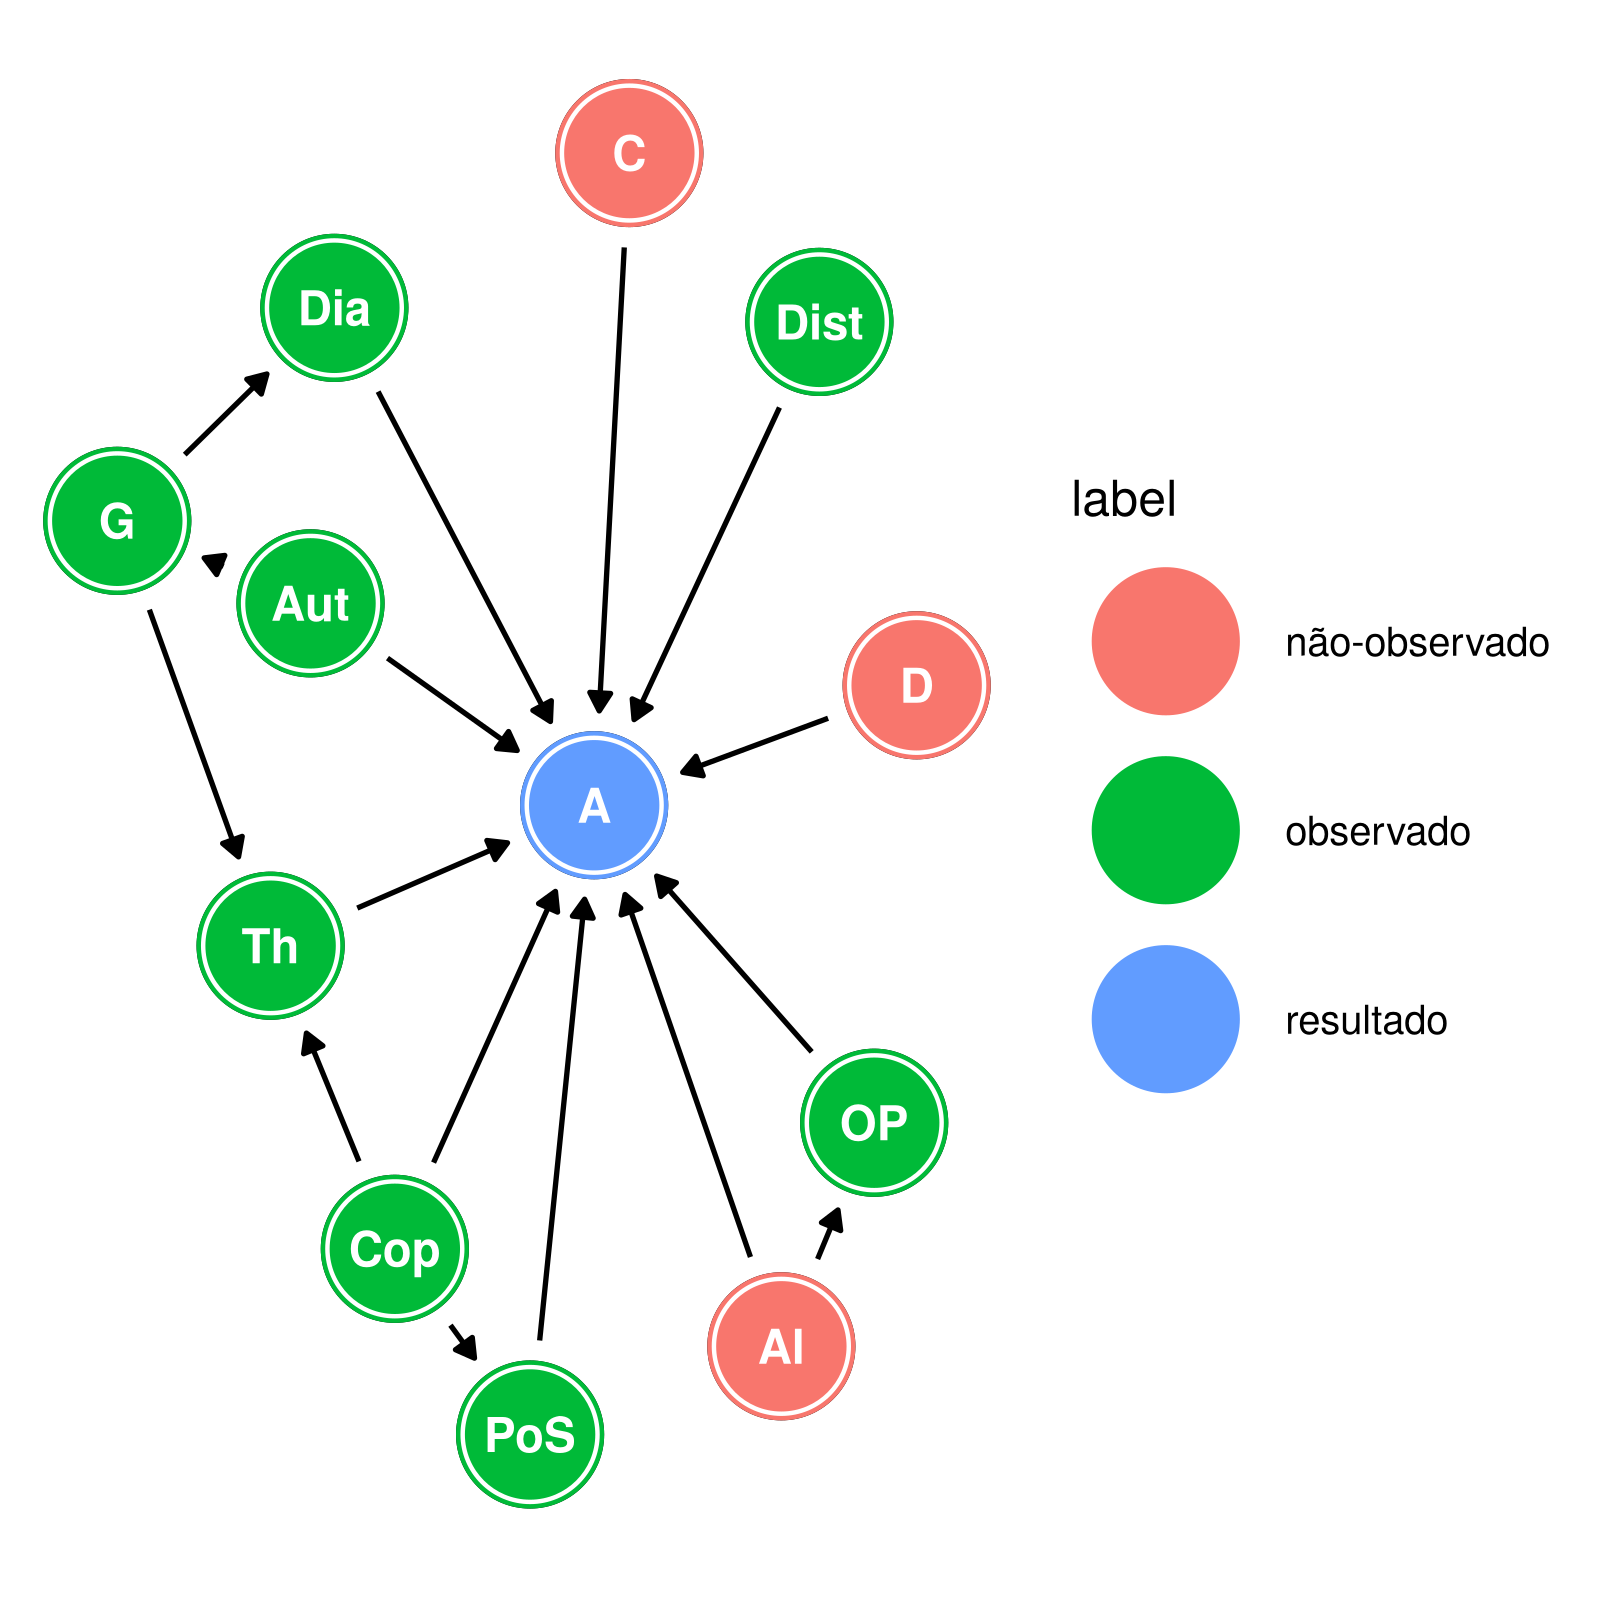
\includegraphics[width=\linewidth]{../fala/plots/dag_d.png}
    \end{center}
    \caption{DAG with \textbf{A}ttraction, \textbf{D}omain, \textbf{C}ontroller,
      \textbf{T}arget,
      \textbf{P}art \textbf{o}f \textbf{S}preech, \textbf{C}opula,
      \textbf{Th}ematic role, \textbf{Auth}orship, \textbf{Genre},
      \textbf{Dia}lect, \textbf{Dist}ance, and \textbf{W}ord \textbf{O}rder.
    }
  \end{minipage}
\end{figure}


\clearpage
\paragraph{Modelo causal final:}
\begin{center}
  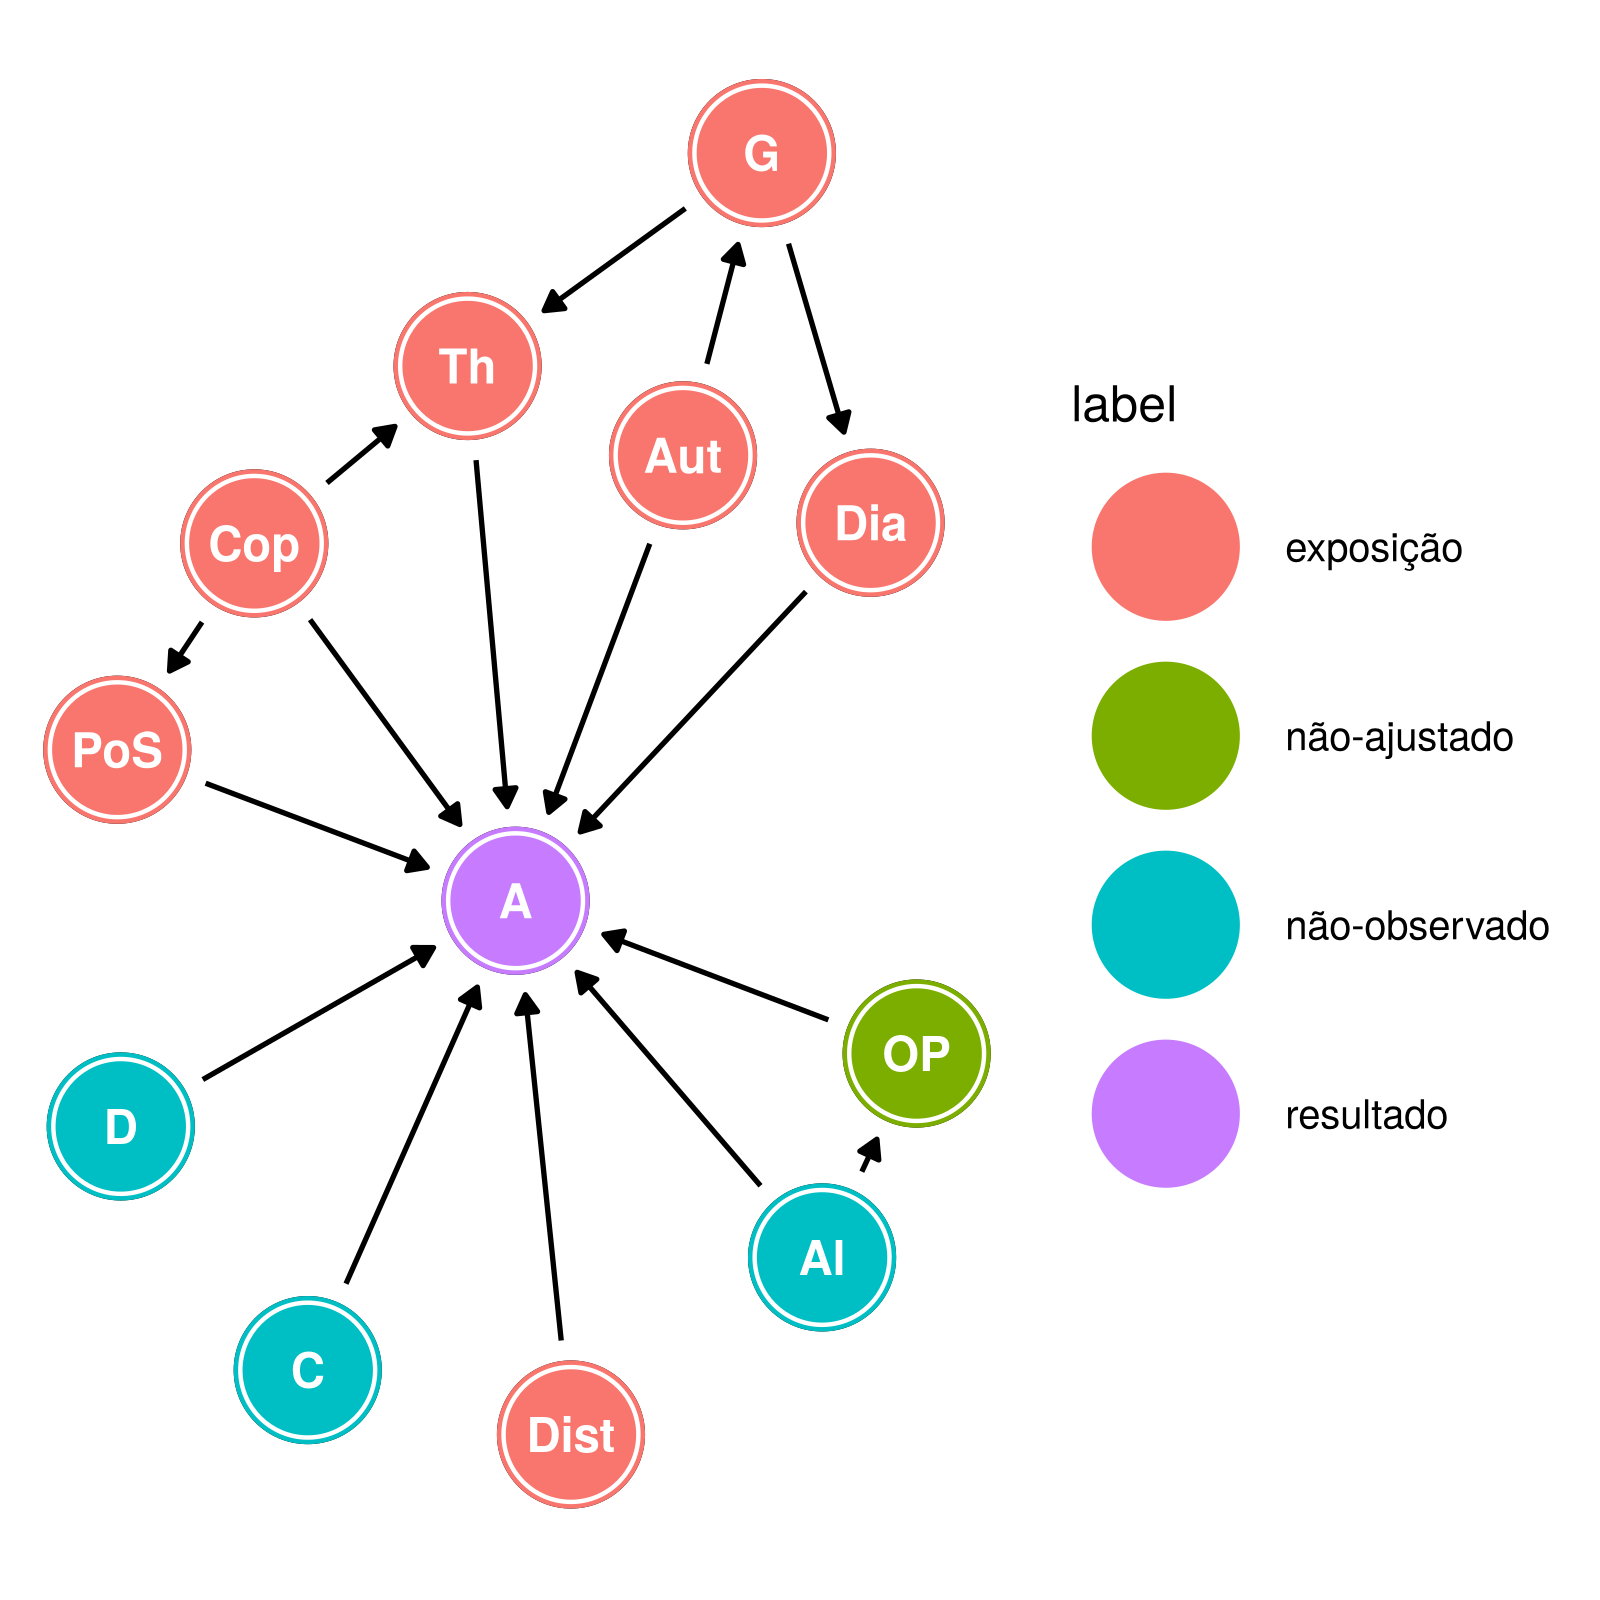
\includegraphics[width=0.7\linewidth]{../fala/plots/dag_e.png}
\end{center}



\paragraph{Modelo linear generalizado:}
\begin{align*}
  \text{A}                                                & \sim \Bernoulli(p_i)                                     \\
  \logit(p_i)                                             & = \alpha_{\Sent} + \bv{Cop}\Cop_i + \bv{Dist}|\Dist_i| + \\
                                                          & + \bv{PoS}\sum^{\PoS_{i}-1}_{j=0}{\delta_{j_{\PoS}}}     \\
                                                          & + \bv{Th}\sum^{Th_{i}-1}_{j=0}{\delta_{j_{\Th}}}         \\
                                                          & + \bvi{Auth} + \bvi{Dia}                                 \\
  \alpha                                                  & = \abar_\Sent + z_{\Sent} * \sigma_\Sent                 \\
  \bv{Cop}, \bv{Dist}                                     & \sim \Normal(0, 1)                                       \\
  \bv{PoS}, \bv{Th}                                       & \sim \Normal(0, 1)                                       \\
  \delta_{\PoS}, \delta_{\Th}                             & \sim \Dirichlet(2)                                       \\
  \bv{Auth}                                               & = z_{\Auth}*\sigma_{\Auth}                               \\
  \bv{Dia}                                                & = \bbar_\Dia + z_{\Dia}*\sigma_{\Dia}                    \\
  \abar_\Sent, \bbar_\Dia, z_{\Sent}, z_{\Auth}, z_{\Dia} & \sim \Normal(0,1)                                        \\
  \sigma_{\Sent}, \sigma_{\Auth}, \sigma_{\Dia}           & \sim \Exponencial(1)
\end{align*}

\paragraph{Cópula e distância} % (fold)

\begin{center}
  
\begin{tabular}[t]{lrrrrr}
\toprule
Effect & mean & sd & 5.5\% & 94.5\% & rhat\\
\midrule
$\beta_{\text{Copula}}$ & 1.81 & 0.47 & 1.07 & 2.57 & 1.00\\
$\beta_{\text{Dist}}$ & -0.27 & 0.06 & -0.37 & -0.18 & 1.01\\
\bottomrule
\end{tabular}

\end{center}



\paragraph{Classe de palavra e hierarquia de predicado} % (fold)

\begin{center}
  
\begin{tabular}[t]{lrrrrr}
\toprule
Effect & mean & sd & 5.5\% & 94.5\% & rhat\\
\midrule
$\beta_{\text{PoS}}$ & 0.76 & 0.51 & 0.17 & 1.71 & 1\\
$\delta_{\text{Adj}}$ & 0.48 & 0.18 & 0.19 & 0.78 & 1\\
$\delta_{\text{Noun}}$ & 0.52 & 0.18 & 0.22 & 0.81 & 1\\
\bottomrule
\end{tabular}

  \bigskip
  
\begin{tabular}[t]{llrrrrr}
\toprule
PoS & Cummulative effect & mean & sd & 5.5\% & 94.5\% & rhat\\
\midrule
Participle & $\beta_{\text{PoS}} * 0$ & 0.00 & 0.00 & 0.00 & 0.00 & --\\
Adjective & $\beta_{\text{PoS}} * \delta_{\text{Adj}}$ & 0.35 & 0.26 & 0.06 & 0.86 & 1\\
Noun & $\beta_{\text{PoS}} * (\delta_{\text{Adj}} + \delta_{\text{Noun}})$ & 0.76 & 0.51 & 0.17 & 1.71 & 1\\
\bottomrule
\end{tabular}

\end{center}

\paragraph{Papel temático do controlador} % (fold)
\begin{center}
  
\begin{tabular}[t]{lrrrrr}
\toprule
Effect & mean & sd & 5.5\% & 94.5\% & rhat\\
\midrule
$\beta_{\text{Theta}}$ & 2.73 & 0.60 & 1.88 & 3.76 & 1\\
$\delta_{\text{Exp}}$ & 0.38 & 0.12 & 0.19 & 0.57 & 1\\
$\delta_{\text{Agent}}$ & 0.62 & 0.12 & 0.43 & 0.81 & 1\\
\bottomrule
\end{tabular}

  \bigskip
  
\begin{tabular}[t]{llrrrrr}
\toprule
Theta & Cummulative effect & mean & sd & 5.5\% & 94.5\% & rhat\\
\midrule
Recipient & $\beta_{\text{Th}} * 0$ & 0.00 & 0.00 & 0.00 & 0.00 & --\\
Experiencer & $\beta_{\text{Th}} * \delta_{\text{Exp}}$ & 1.04 & 0.41 & 0.44 & 1.73 & 1\\
Agent & $\beta_{\text{Th}} * (\delta_{\text{Exp}} + \delta_{\text{Agent}})$ & 2.73 & 0.60 & 1.88 & 3.76 & 1\\
\bottomrule
\end{tabular}

\end{center}

\begin{figure}[!h]
  \centering
  \begin{minipage}{.48\textwidth}
    \centering
    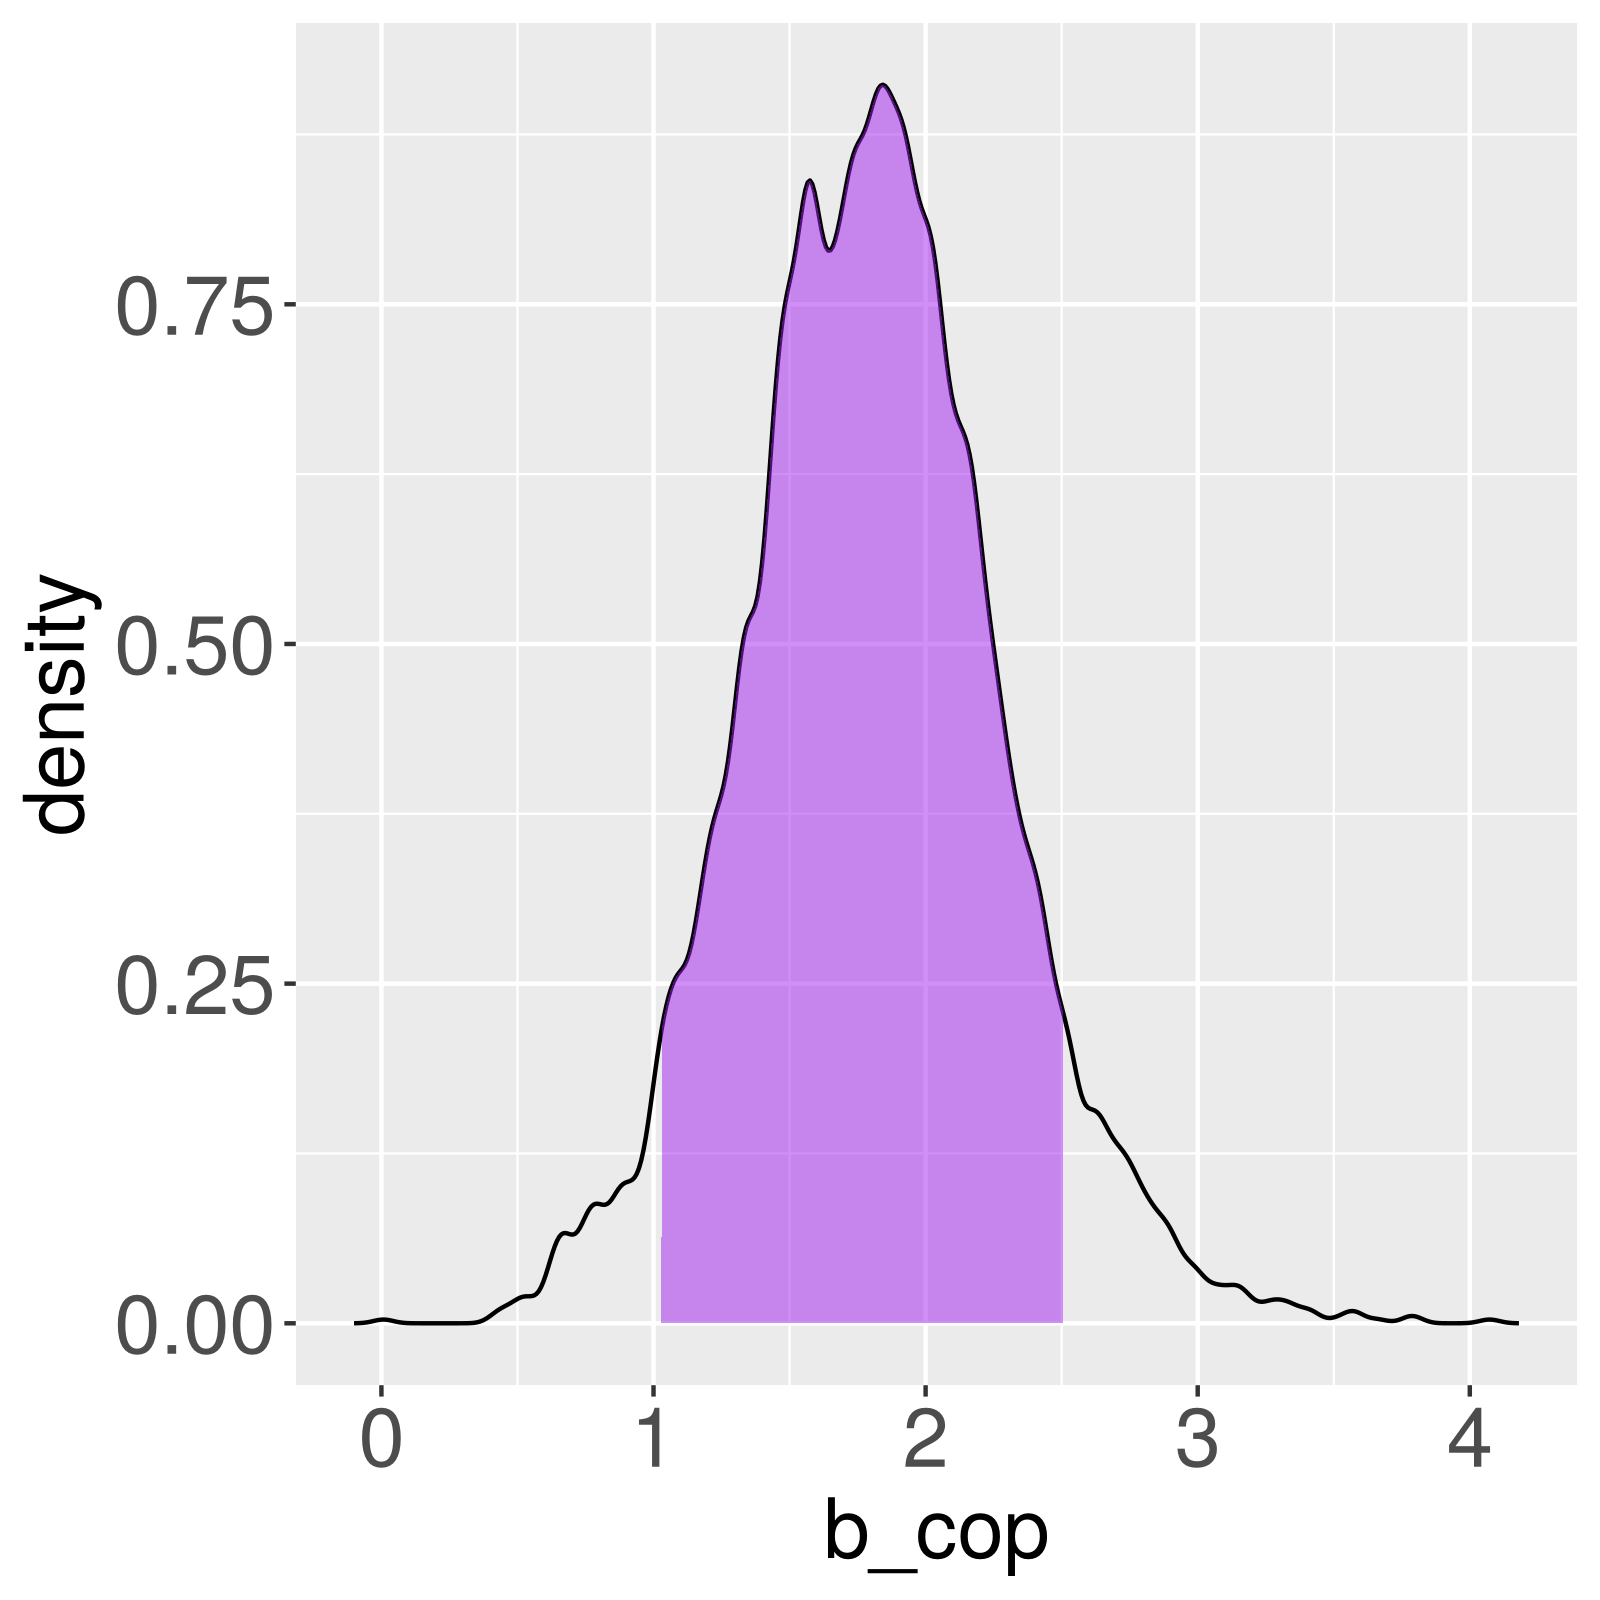
\includegraphics[width=\linewidth]{../fala/plots/posterior_b_copula.png}
    \captionof{figure}{Distribuição posterior de $\beta_\text{Cop}$ com o 89\% do
      Intervalo de Maior Densidade Posterior.}
  \end{minipage}%
  \hfill
  \begin{minipage}{.48\textwidth}
    \centering
    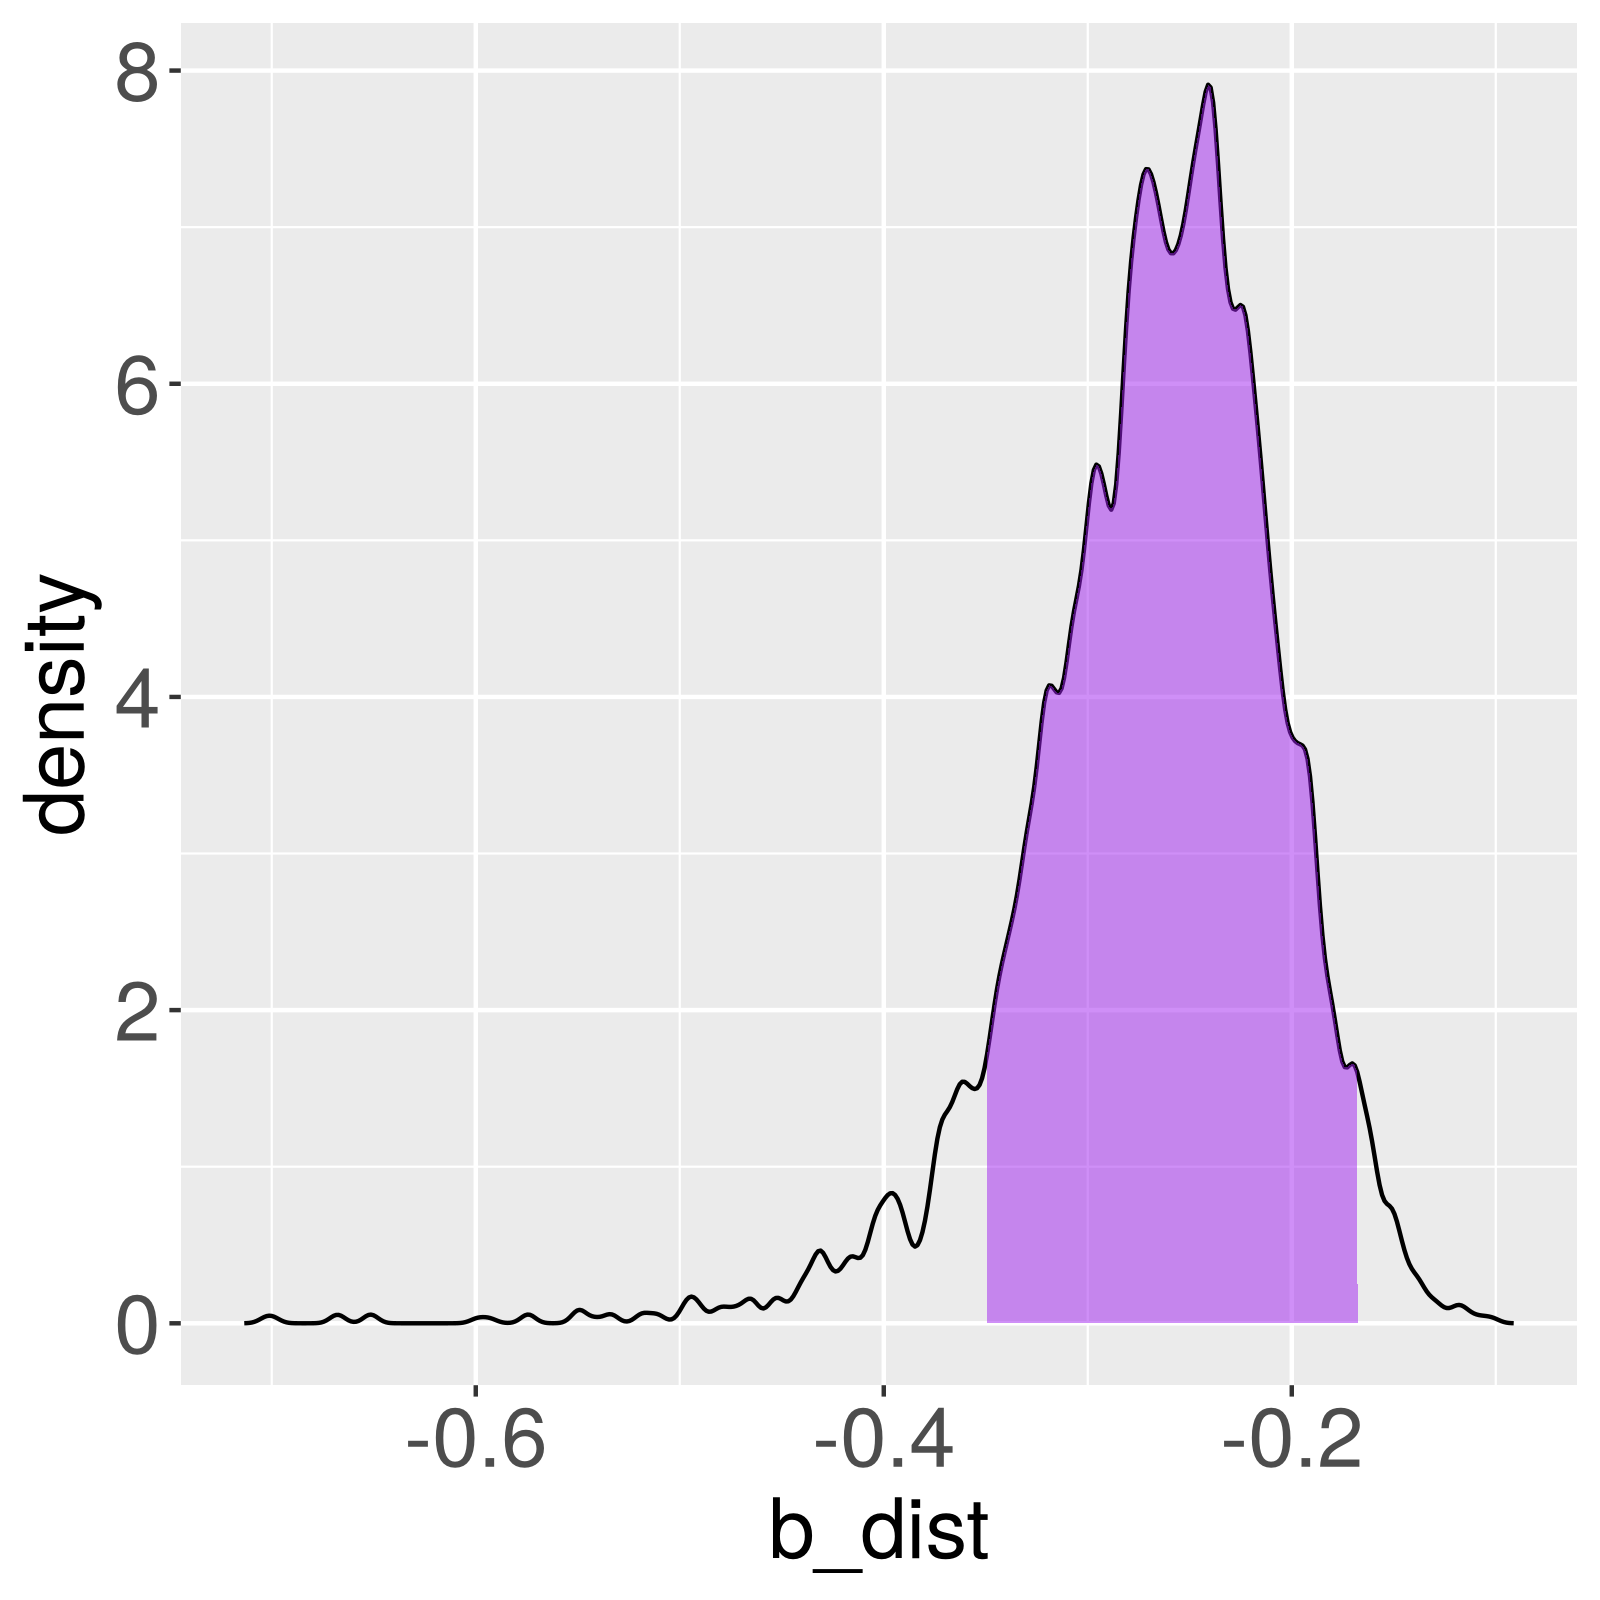
\includegraphics[width=\linewidth]{../fala/plots/posterior_b_dist.png}
    \captionof{figure}{Distribuição posterior de $\beta_\text{Dist}$ com o 89\% do
      Intervalo de Maior Densidade Posterior.}
  \end{minipage}
\end{figure}
\begin{figure}[!h]
  \centering
  \begin{minipage}{.48\textwidth}
    \centering
    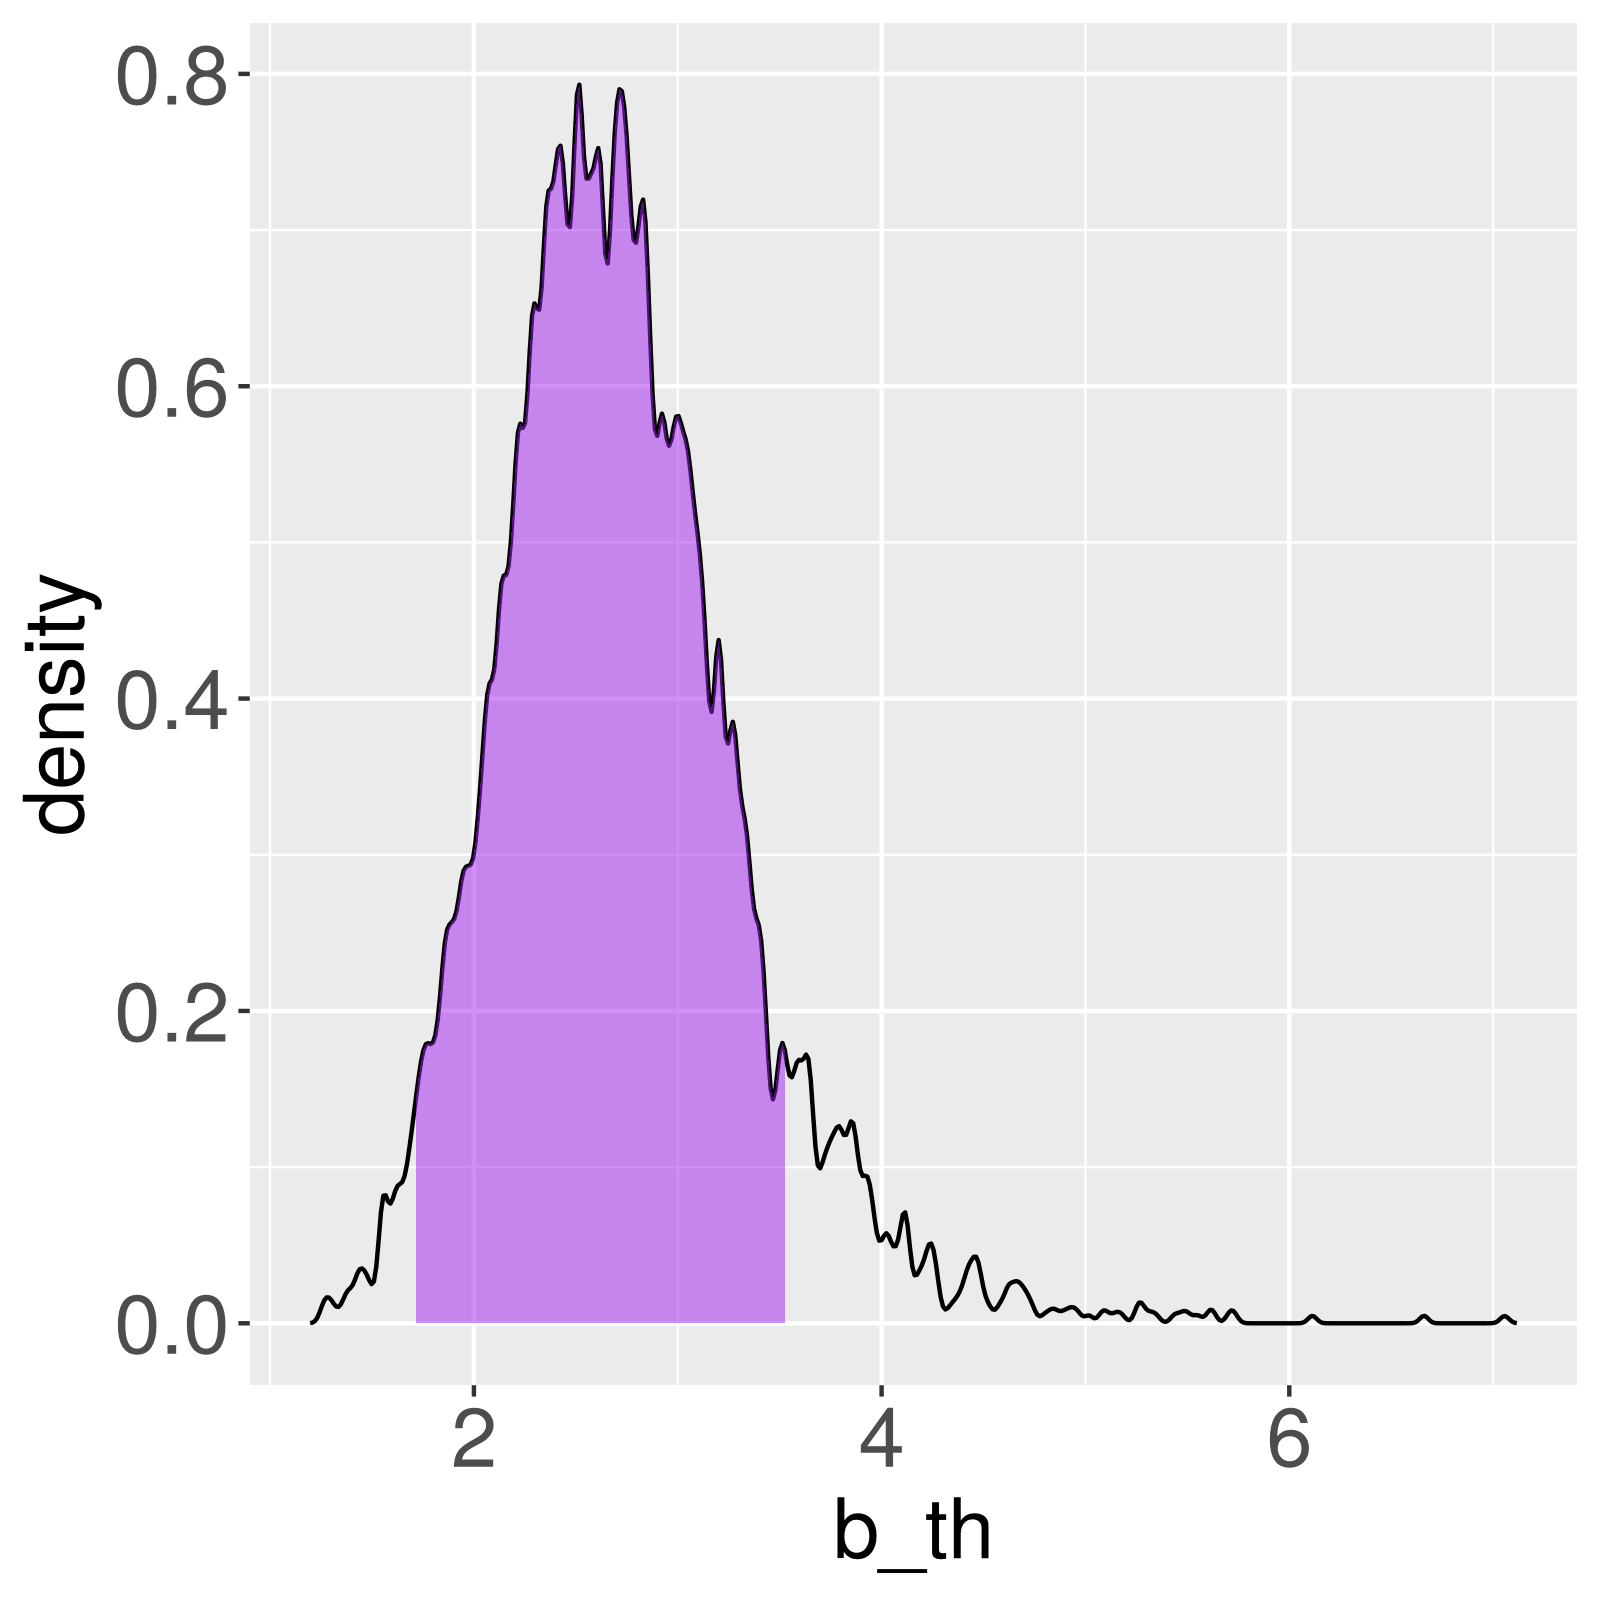
\includegraphics[width=\linewidth]{../fala/plots/posterior_b_th.png}
    \captionof{figure}{Distribuição posterior de $\beta_\text{Th}$ com o 89\% do
      Intervalo de Maior Densidade Posterior.}
  \end{minipage}%
  \hfill
  \begin{minipage}{.48\textwidth}
    \centering
    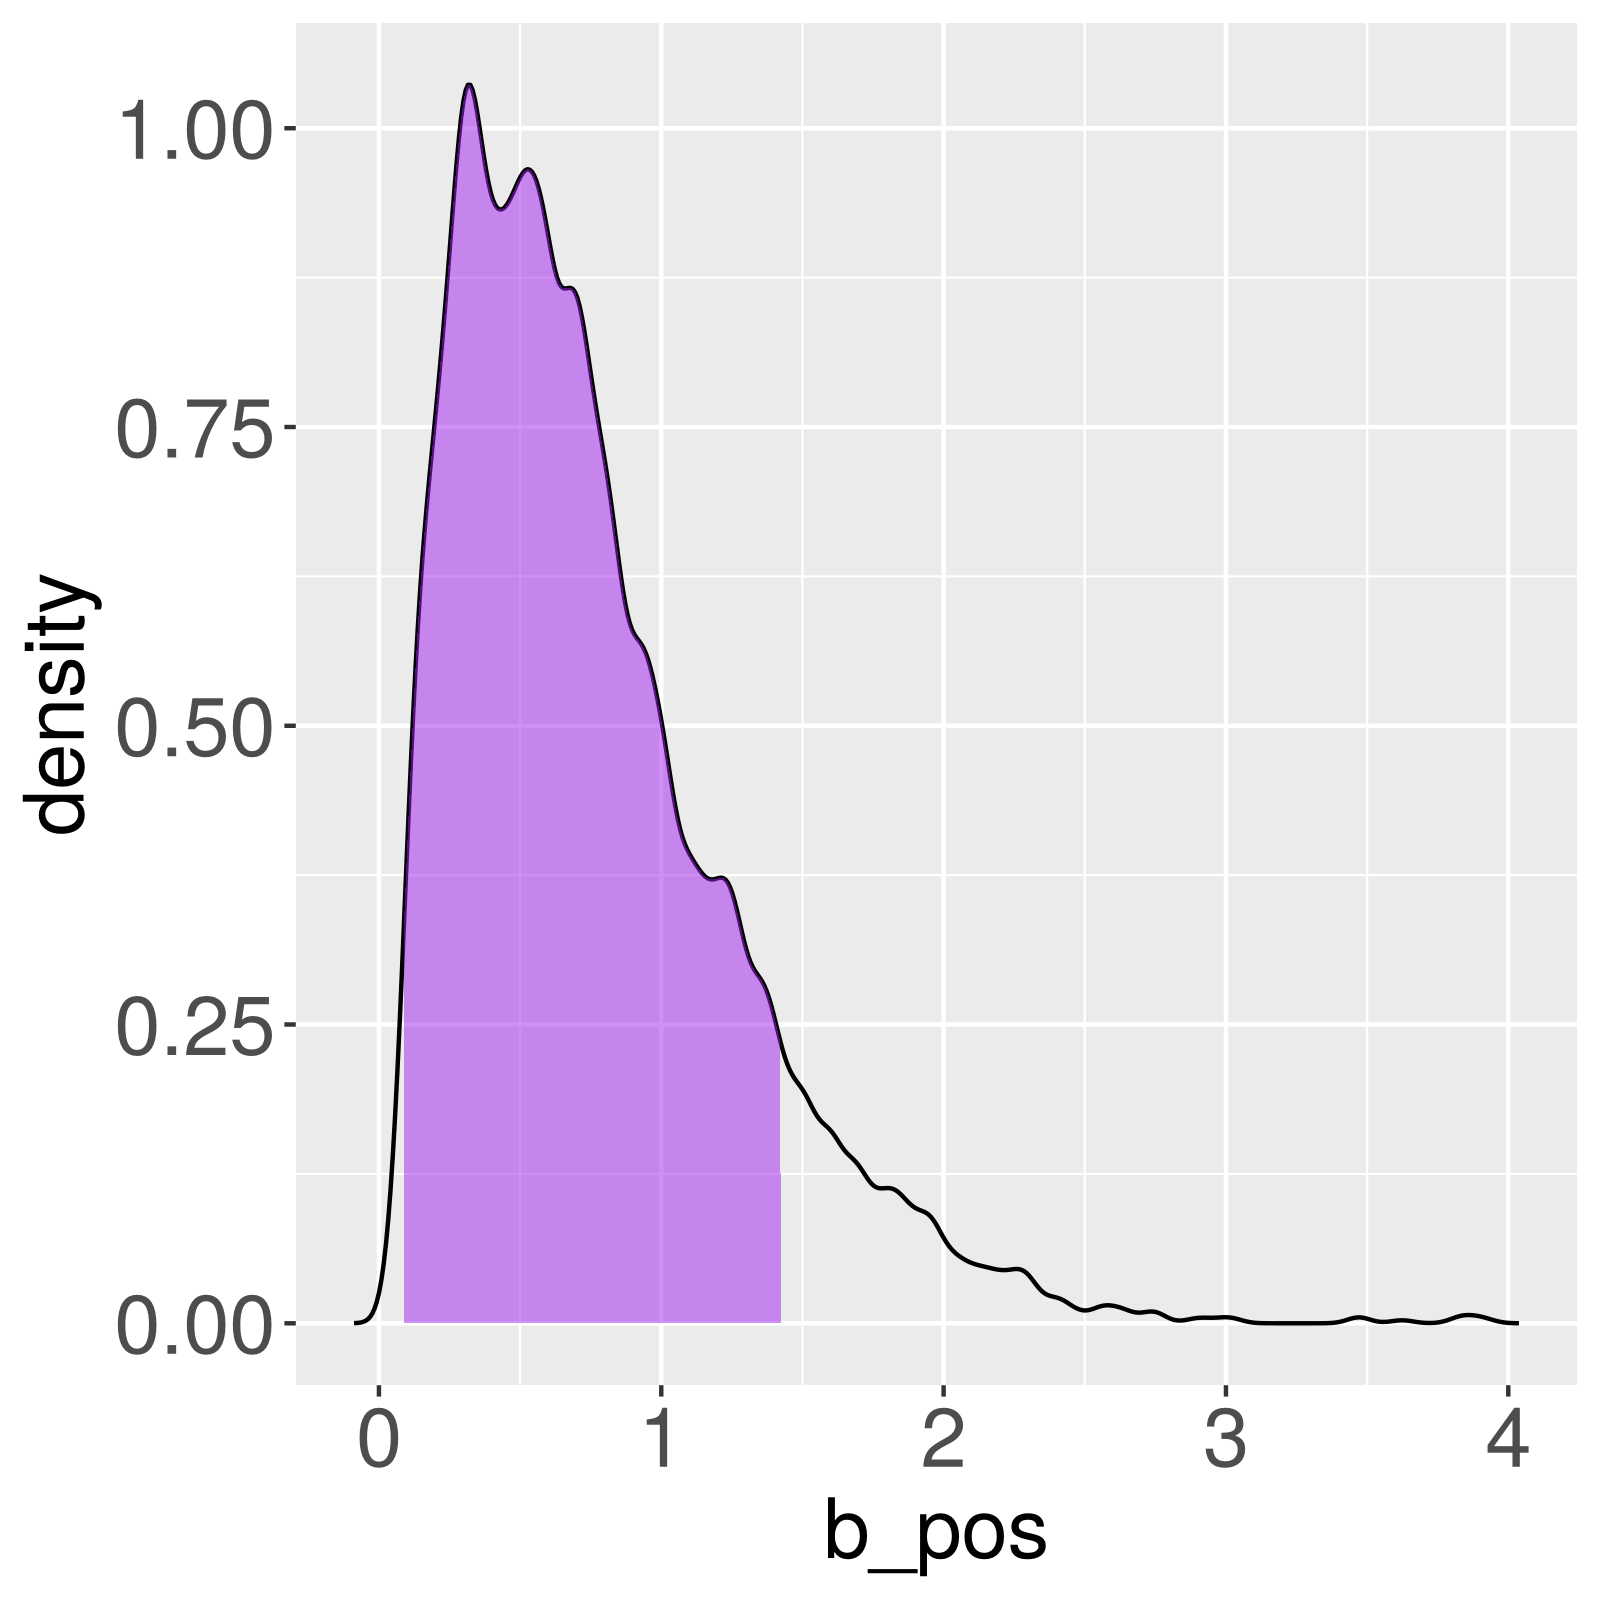
\includegraphics[width=\linewidth]{../fala/plots/posterior_b_pos.png}
    \captionof{figure}{Distribuição posterior de $\beta_\text{PoS}$ com o 89\% do
      Intervalo de Maior Densidade Posterior.}
  \end{minipage}
\end{figure}

\clearpage
\paragraph{Dialeto e Autoria} % (fold)

\begin{center}
  
\begin{tabular}[t]{lrrrrr}
\toprule
Effect & mean & sd & 5.5\% & 94.5\% & rhat\\
\midrule
$\overline{\beta}_{\text{Dia}}$ & -0.37 & 0.80 & -1.64 & 0.93 & 1\\
$\sigma_{\text{Dia}}$ & 1.33 & 0.86 & 0.27 & 2.90 & 1\\
$\beta_{\text{Attic}}$ & 0.13 & 0.87 & -1.26 & 1.50 & 1\\
$\beta_{\text{Jonic}}$ & -1.60 & 1.14 & -3.50 & 0.17 & 1\\
$\beta_{\text{Attic}} - \beta_{\text{Jonic}}$ & 1.73 & 0.94 & -0.04 & 3.01 & --\\
\bottomrule
\end{tabular}

\end{center}

\begin{figure}[!h]
  \centering
  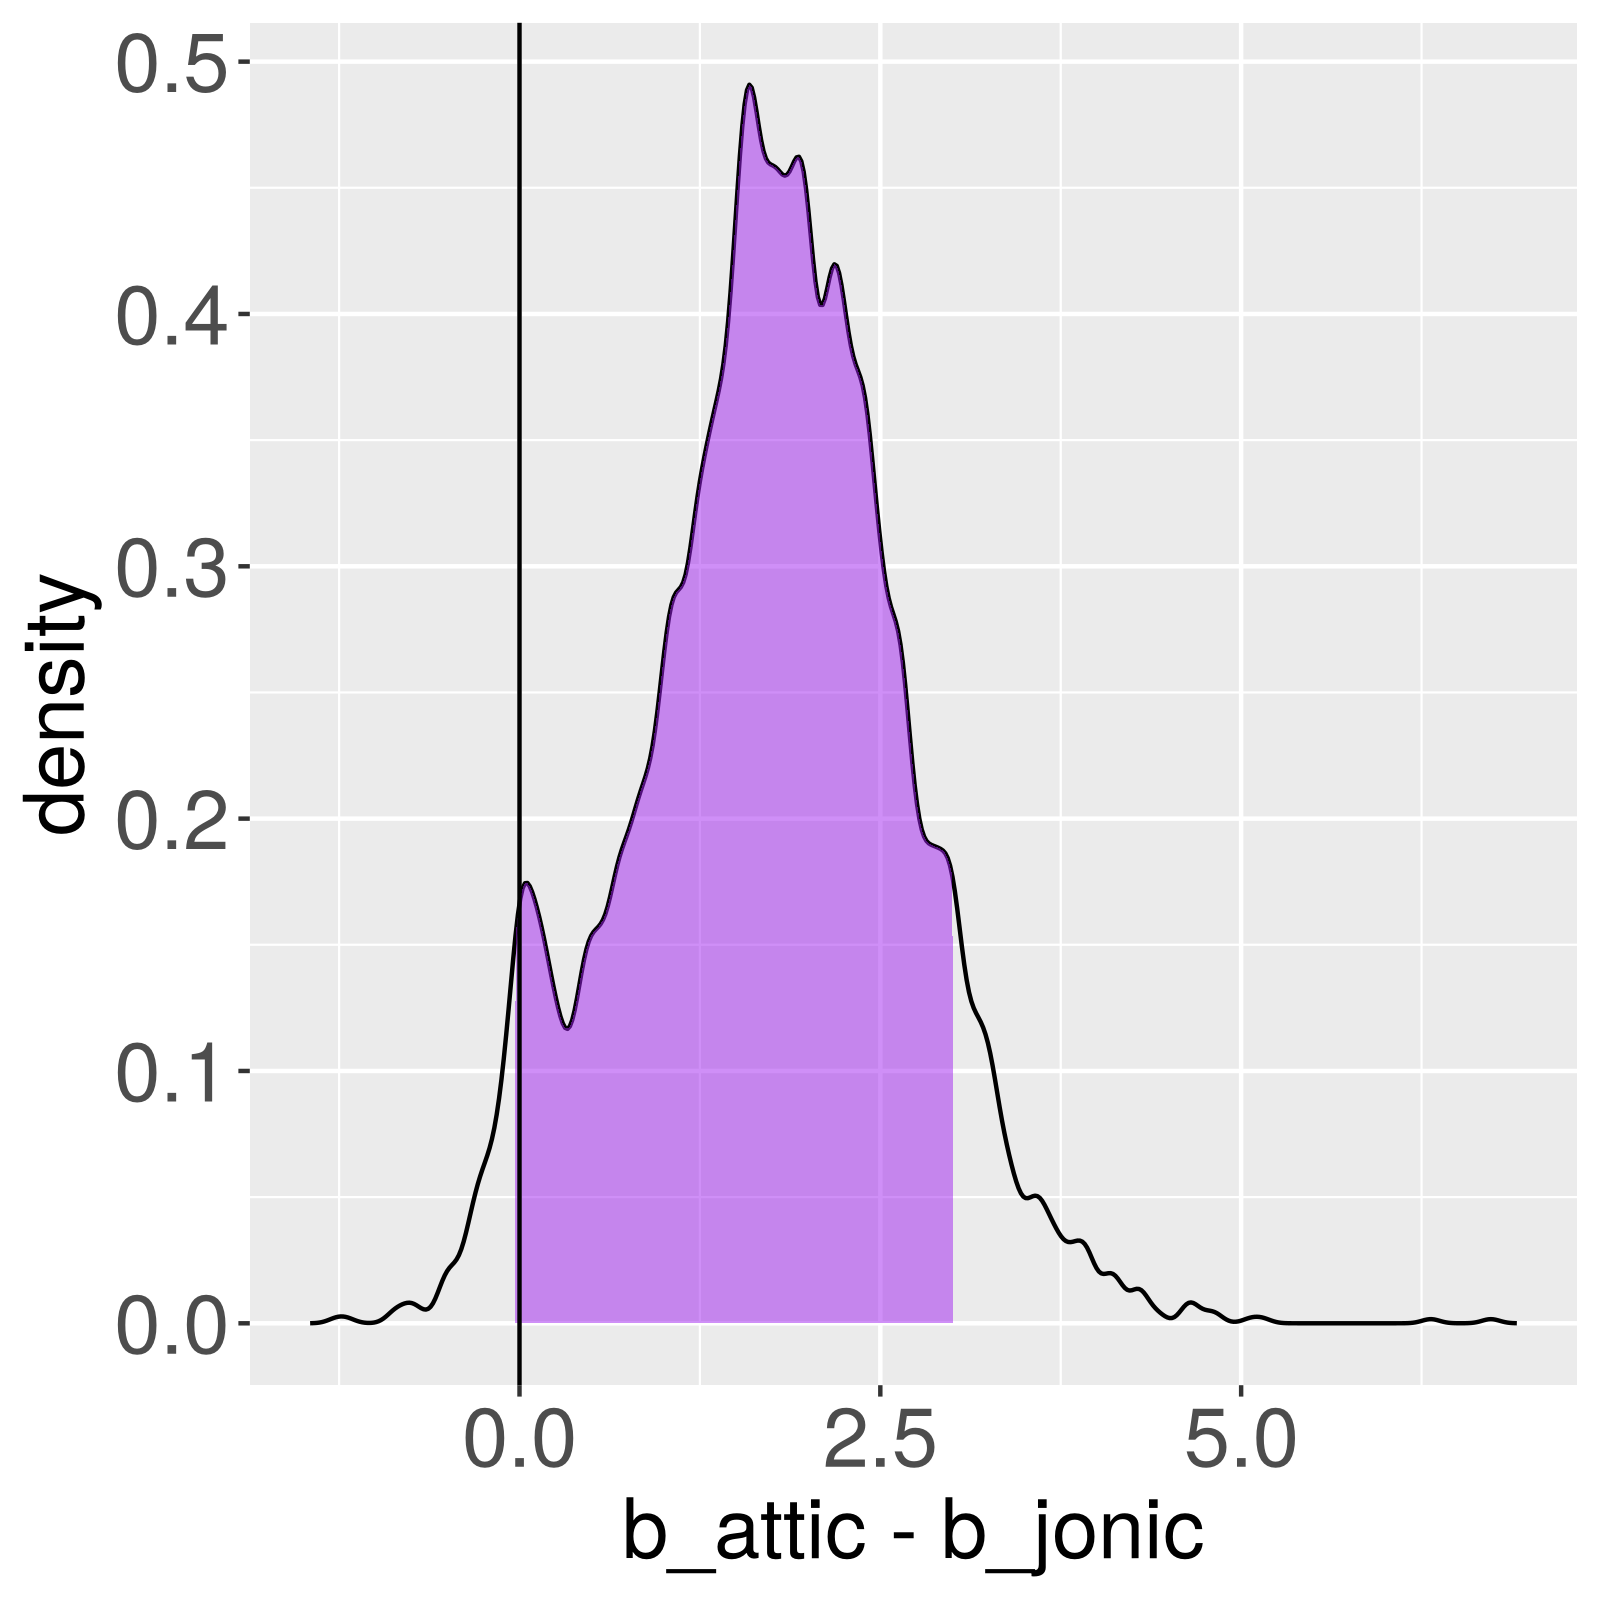
\includegraphics[width=0.45\linewidth]{../fala/plots/posterior_diff_dia.png}
  \caption{Distribuição posterior da diferença entre
    $\beta_\text{Attic}$ e $\beta_\text{Jonic}$ com o 89\% do
    Intervalo de Maior Densidade Posterior.}
\end{figure}

\begin{figure}[!h]

  \begin{center}
    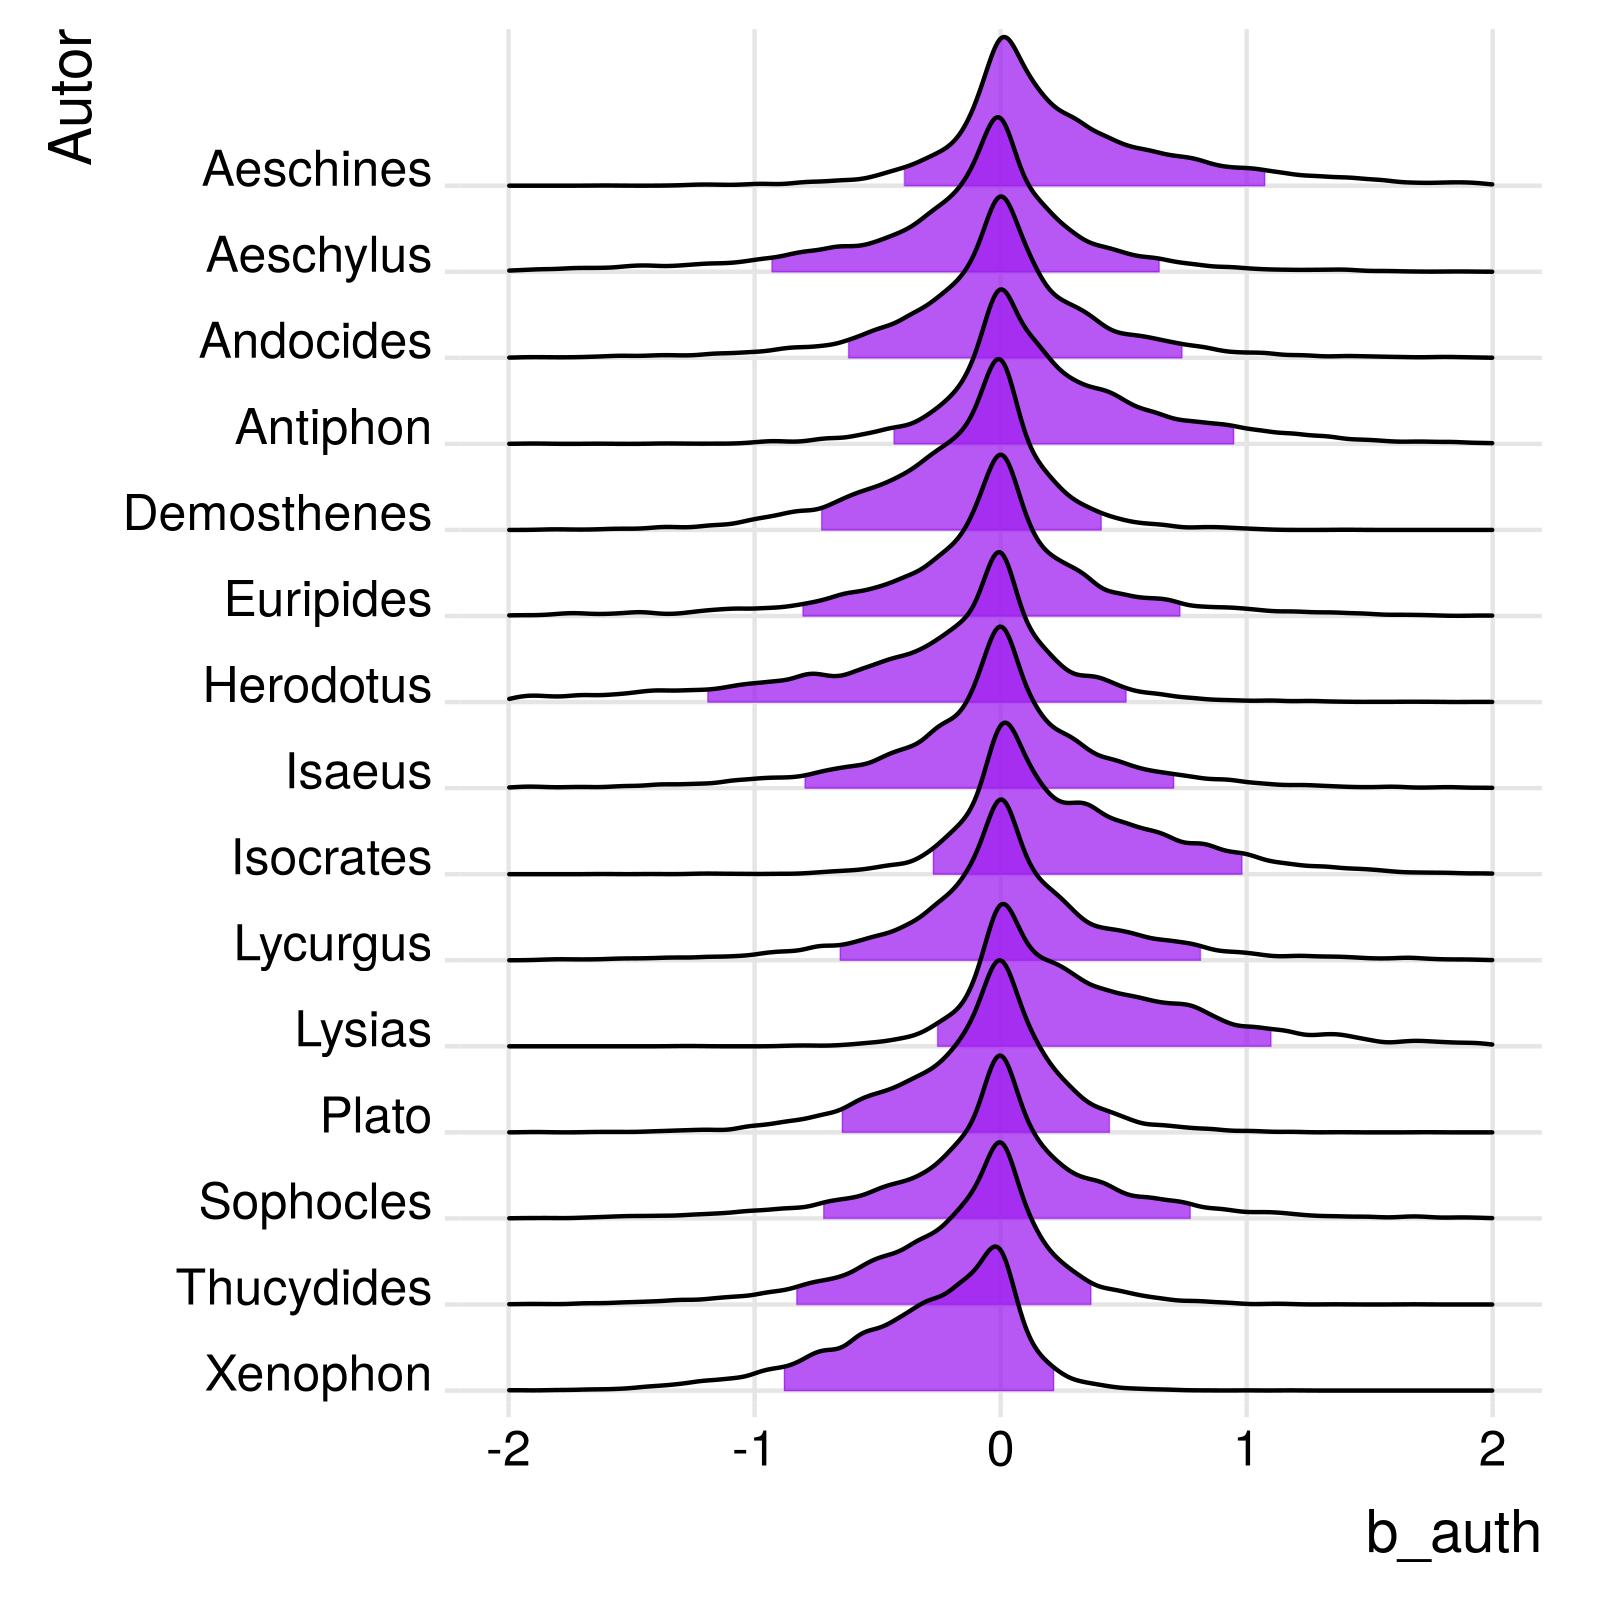
\includegraphics[width=0.70\linewidth]{../fala/plots/dens_authors.png}
  \end{center}
  \caption{Distribuição posterior dos efeitos de autoria
    com o 89\% do
    Intervalo de Maior Densidade Posterior.}
\end{figure}

\clearpage
\renewcommand*{\mkbibnamefamily}[1]{\textsc{#1}}
\printbibliography%
\renewcommand*{\mkbibnamefamily}[1]{#1}

\end{document}
